\documentclass[12pt,twoside,headsepline,titlepage]{thesis}
\usepackage{algorithm}
\usepackage{algpseudocode}
\usepackage{caption}
\usepackage[usenames]{color}
\usepackage[table]{xcolor}
\usepackage{graphicx}
\usepackage[bookmarks,backref=true,linkcolor=black]{hyperref} %,colorlinks
\usepackage{listings}
\usepackage{mathptmx}
\usepackage[absolute]{textpos}
\usepackage{times}
\usepackage{tikz}
\usetikzlibrary{arrows,positioning,shadows,shapes}
\usepackage{url}

\tikzstyle{state} = [draw, fill=blue!10, text width=4.00em, text
                     centered, node distance=2.6cm, inner sep=0.5em, rounded
%                     corners, minimum height=3em, circular drop shadow]
                     corners, minimum height=3em, drop shadow]
\tikzstyle{line} = [draw, ultra thick, -latex]

\DeclareGraphicsExtensions{.pdf,.png,.jpg}
%
% jens-macros.tex
%

%% Jens: improve typesetting quality
\usepackage{microtype}

%% Jens: Color include, needed for some of the macros below
\usepackage[usenames]{color}
%% Jens: The \anonymizeForReview macro automatically replaces text with the word
%%       "anonymized" in bold gray if a "review" documentclass is choosen
%%        otherwise it's a NOOP
%\ifreviewelse{\newcommand{\anonymizeForReview}[1]{\textcolor[rgb]{0.50,0.50,0.50}{\textbf{anonymized}}}}{\newcommand{\anonymizeForReview}[1]{#1}}
%% Jens: The \TODO macro is used to flag text that should
%%       not make it into the submitted version, it is
%%       compiled to red text and should also be easy to
%%       find by a search call in the tex file before
%%       submission.
\newcommand{\TODO}[1]{\textcolor[rgb]{1.00,0.00,0.00}{\textbf{#1}}}
\newcommand{\todo}[1]{\textcolor[rgb]{1.00,0.00,0.00}{\textbf{#1}}}
%\newcommand{\TODO}[1]{}
%% Jens: Helper for the \CE macro below
\makeatletter
\def\ifEmpty#1{\def\@temp{#1}\ifx\@temp\@empty}
\makeatother
%% Jens: The the \isDraft macro to true to replace all images by
%%       (correctly sized) boxes for faster preview
\newcommand{\isDraft}{false}
%% Jens: for align environment
\usepackage{amsmath,amsfonts,amssymb}
%% for using urls
\definecolor{darkblue}{rgb}{0,0,0.75}
%% Jens: get rid of the ifpdf clash (needed for the hyperrefs below)
\makeatletter
\let\saved@ifpdf\ifpdf
\let\ifpdf\@undefined
\usepackage{ifpdf}
%\let\ifpdf\saved@ifpdf
%\makeatother
%% Jens: turn refs into links and give them a blue color (remove for print version)
%%\usepackage[colorlinks=true,linkcolor=darkblue,citecolor=darkblue,urlcolor=darkblue]{hyperref}
%% Jens: Define a new 'tinyurl' style for the package that will use a smaller font.
%%       this can be activated in the references by inserting: \urlstyle{tinyurl}
%\makeatletter

\usepackage{graphics,graphicx}

% Math Commands
\newcommand{\mat}[1] {\boldsymbol{#1}} %{#1}
\newcommand{\vect}[1]{\boldsymbol{#1}}
\newcommand{\uvect}[1]{\boldsymbol{\hat{#1}}}
\newcommand{\norm}[1]{\lVert#1\rVert}
\newcommand{\abs}[1]{\lvert#1\rvert}
\newcommand{\transp}[1]{{#1}^\top}
\newcommand{\invtransp}[1]{{#1}^{-\top}}
\newcommand{\inv}[1]{{#1}^{-1}}
\newcommand{\scprod}[2]{#1\cdot#2}
\newcommand{\inprod}[2]{\left<#1,#2\right>}
\newcommand{\real}{\mathbb{R}}
\newcommand{\rthree}{\reel^3}
\newcommand{\cmplx}{\mathbb{C}}
\newcommand{\ints}{\mathbb{Z}}
\newcommand{\conj}[1]{\overline{#1}}

\newcommand{\SC}[1]{Sec.~\ref{#1}}
\newcommand{\SCp}[1]{Section~\ref{#1} on page~\pageref{#1}}
\newcommand{\EQWB}[1]{(Eq.~\ref{#1})}
\newcommand{\EQ}[1]{Eq.~\ref{#1}}
\newcommand{\EQp}[1]{Equation~\ref{#1} on page~\pageref{#1}}
\newcommand{\FG}[1]{Fig.~\ref{#1}}
\newcommand{\FGp}[1]{Figure~\ref{#1} on page~\pageref{#1}}
\newcommand{\TA}[1]{Table~\ref{#1}}
\newcommand{\TAp}[1]{Table~\ref{#1} on page~\pageref{#1}}
\newcommand{\AL}[1]{Algorithm~\ref{#1}}
\newcommand{\ALp}[1]{Algorithm~\ref{#1} on page~\pageref{#1}}

\DeclareMathOperator{\sinc}{sinc}
\DeclareMathOperator{\mmid}{mid}
\DeclareMathOperator{\sincBCC}{sincBCC}
\DeclareMathOperator{\ramp}{\mathcal{R}}
\DeclareMathOperator{\boxx}{\mathcal{B}}
\DeclareMathOperator{\step}{\mathcal{H}} %{Heaviside}
\DeclareMathOperator{\tesseract}{\mathcal{T}}
\DeclareMathOperator{\hatfcn}{\Lambda}
\DeclareMathOperator{\grad}{\nabla}
\newcommand{\Fourier}[1]{\mathcal{F}\{#1\}}
\newcommand{\shah}{{\textstyle \amalg{\kern-4.pt\amalg}}}
\newcommand{\myx}[1]{{x}_#1}
\newcommand{\myy}[1]{{y}_#1}
\newcommand{\myz}[1]{\mathrm{z}_#1}
\newcommand{\myw}[1]{\mathrm{w}_#1}
\newcommand{\myxi}[1]{\vect{\xi}_#1^\perp}
% I really hate TeX sometimes.
\newcommand{\tjftilde}{\raise.17ex\hbox{$\scriptstyle\mathtt{\sim}$}}

\newcommand{\tjfsec}[1]{Section~\ref{#1}}
%\newcommand{\tjfsec}[1]{\S{\ref{#1}}}

\title{Visualizing and understanding large regular data}

\begin{document}

\begin{titlepage}
\vspace*{-1cm}
\newlength{\links}
\setlength{\links}{0.9cm}
\setlength{\TPHorizModule}{1cm}
\setlength{\TPVertModule}{1cm}
%\textblockorigin{0pt}{0pt}

\sf
\LARGE

\begin{textblock}{16.5}(2.8,2.7)
 \hspace*{-0.8cm} \textbf{University of Duisburg-Essen} \\
 \hspace*{-1.15cm} \rule{5mm}{5mm} \hspace*{0.0cm} Faculty of Engineering\\
 \large{}Department of Computer and Cognitive Sciences\\
\end{textblock}

%Hier Titel, Name, und Matrikelnummer eintragen, \\ make a newline
\begin{textblock}{14.5}(3.2,7.5)
\begin{center}
  \large
{\bf Doctoral Dissertation} \\[1cm]
{ \LARGE  \bf Visualizing and understanding large regular data} \\[1.3cm]
Thomas Fogal\\
Matriculation Number: 300306200
\end{center}
\end{textblock}

\begin{textblock}{10}(10.5,15.5)
\includegraphics[width=.94\textwidth]{images/unilogo}\\
\normalsize
\raggedleft
Department of Computer and Cognitive Sciences \\
Faculty of Engineering \\
University of Duisburg-Essen \\[2ex]

\today\\[13ex]
%February 28, 2015\\[13ex]
\raggedright
% Supervisors
{\bf Supervisor:} \\
Prof. Dr. rer. nat. Jens Kr\"uger\\

{\bf Reviewers:}\\
Prof. Dr. rer. nat. Jens Kr\"uger\\
Prof. Chris Johnson\\
%\todo{Prof. Dr. J\"urgen Ziegler ??}\\
%\todo{????}
\end{textblock}

\end{titlepage}

%
% additional declaration
%

\clearpage
\thispagestyle{empty}
~
% \vfill
\begin{flushleft}
  \textbf{Eidesstattliche Versicherung / Statement in lieu of an oath:}\\
  Ich versichere hiermit an Eides Statt, dass ich die vorliegende
  Arbeit selbstst\"andig verfasst und keine anderen als die angegebenen
  Quellen und Hilfsmittel verwendet habe.\\

  I hereby confirm that I have written this dissertation on my own
  and that I have not used any media or materials other than the ones
  referred to in this dissertation.\\[\baselineskip]

	Santa Clara, CA, USA\\
	\today{}\\%February 28, 2015\\

% \vspace{4cm}
% 	\textbf{Einverst\"andniserkl\"arung / Declaration of Consent:}\\
% 	Ich bin damit einverstanden, dass meine (bestandene) Arbeit in beiden Versionen in die Bibliothek der
% Informatik aufgenommen und damit ver\"offentlicht wird.\\
% 	I agree to make both versions of my thesis (with a passing grade) accessible to the public by having
% them added to the library of the Computer Science Department.\\[\baselineskip]
% 	Duisburg, August 01, 2014
% \vspace{3cm}
\end{flushleft}

\clearpage

\section*{Zusammenfassung / Abstract}

Die Visualisierung ist ein wesentlicher Bestandteil, wenn es um das
Verstehen enorm gro\ss{}er Datenmengen geht, die sowohl in Simulationen
als auch durch bildgebende Verfahren wie die Computertomographie
entstehen k\"onnen. Die Anordnung dieser Daten bestimmt hierbei,
wie diese algorithmisch verarbeitet werden k\"onnen, und hat somit
Einfluss auf die Effizienz derjeniger Prozesse, die auf solchen Daten
operieren. Aus diesen Performanzgr\"unden und auf Grund der Einfachheit
der Implementierung hat die regul\"are $N$D Gitteranordnung die
Bereiche der Simulation, Medizin und Visualisierung dominiert.

Allerdings reicht die regul\"are Anordnung der Daten nicht aus. Die
Geschwindigkeit, mit der die Datenmengen wachsen, \"ubersteigt
den Hardwarewachstum seit vielen Jahren, und die so entstandene
Leistungsabstand sorgt f\"ur Schwierigkeiten im Bereich der
Visualisierungsalgorithmen. Da sich beinahe alle Wissenschaften in
die Richtung von datenzentrierten Verfahren bewegen, stellen diese
Leistungseinschr\"ankungen einen limitierenden Faktor f\"ur den
wissenschaftlichen Fortschritt dar.

Um diese Datenmengen zu bew\"altigen, wird von vielen die sogenannte
\textit{in-situ}-Visualisierung eingesetzt. Dabei werden die
Simulation und die Visualisierung verbunden, um Verz\"ogerungen zu
minimieren. Momentan ist dies ein m\"uhseliger Prozess, welcher auf
Grund von mangelnden
Software-Engineering-Ressourcen nicht im gr\"o\ss{}eren Ausma\ss{} im
akademischen Umfeld durchf\"uhrbar ist.

Diese Dissertation demonstriert einige, durch die Community bereits
\"uberpr\"ufte Ideen, um die genannten H\"urden zu eliminieren. Der
Algorithmus im Fokus ist dabei Volumengrafik, eine weit verbreitete
Methode f\"ur das Datenverst\"andnis in vielen wissenschaftlichen
Disziplinen. W\"ahrend wir an der Problemstellung arbeiten, kombinieren
wir L\"osungen f\"ur Volumengrafik mit
Simulationssoftware auf \textit{in-situ}-Basis und schlagen dabei
verschiedene Wege ein, um besonders den Engineering-Aufwand zu
minimieren.


\vspace{1em}

\hrule{}
\vspace{1em}

Visualization has emerged as a critical component in deriving
understanding from the vast amounts of data generated from both
simulations and modern scanning technologies such as computed
tomography.  The organization of these data dictates how they are
algorithmically processed and thereby the performance of processes
that operate on the data.  For these performance reasons as well as
simplicity of implementation, a regular $N$D grid organization has
heretofore dominated in the simulation, medical, and visualization
domains.

Yet the regular organization of data alone is not enough.  The pace of
data growth has exceeded that of hardware growth for many years now,
and the ensuing performance gap creates difficulties for visualization
algorithms.  As basically all sciences move to a data-centric approach,
these performance limitations become the limiting factor in forward
scientific progress.

To deal with this delude of data, many have turned to \textit{in situ}
visualization: coupling simulation and visualization software together
in an effort to minimize delay.  This is presently a daunting process,
one that cannot be sustained at large scale with the dearth of software
engineering resources across the research community.

This dissertation presents a number of community-vetted ideas aimed at
removing these barriers.  The algorithm targeted is volume rendering,
a popular method for data understanding in a number of scientific
disciplines.  As we dissipate these challenges, we turn to the related
problem of integrating volume rendering solutions with
simulation software \textit{in situ}, specifically focusing on ways to
minimize the engineering investment.

\newpage
\section*{Acknowledgements}

Certainly, the primary acknowledgement should go to my advisor and
friend through this whole endeavor, Jens Kr\"uger.  It would be
impossible to overstate his contribution to this work, from developing
arguments to coding to writing and presenting; you would surely not be
reading this work today, if not for Jens.

A special thanks is also due to Hank Childs.  In addition to
significant contributions in writing the paper associated with
Chapter~\ref{chp:multiscale} and help integrating code with VisIt,
Hank's constant encouragement and praise were often exactly what I
needed to keep pushing after setbacks.

I was fortunate to enjoy a summer at Oak Ridge National Laboratory, the
highlight of which was discussing parallel rendering research with Sean
Ahern, a Chromium author.  I was that kid that set up Chromium in his
dorm room just because `he thought it was cool'; years later, Sean was
gracious enough to pretend I was an equal.  Thanks, Sean.

I am grateful to Gunther Weber and Mark Howison, who helped us identify
the research challenges and questions we wanted to address when our HPG
volume rendering paper was less than an inkling of an idea.
%  Gunther
%and I have had many interesting AMR volume rendering conversations, as
%well.

Chuck Hansen has been especially helpful in helping me to formulate
relevant ideas and present them effectively.  Thanks!

%Chuck offers help
%whenever I ask without delay or expectation of anything in return.

Chris Johnson deserves a special thanks.  He was the perfect manager
while I was at SCI: his door was always open, the research challenges
were always beyond measure, the queue of collaborators grew faster than
it shrank, direction was available but never prescribed, and a golden
road of funding grew wherever I wandered.  Perhaps the best testament
to his style is that it is only now, looking back, that I realize I was
working for him and not myself.

Both Pat McCormick and Matt Might had enlightening insights on the
\textit{in situ} approaches developed in this work.

Special thanks are due to friends in my research group, notably
Alexander Schiewe and Andrey Krekhov, for copious supplies of
sanity-inducing beer.  Wouldn't have been the same without you
guys---thanks.

Some computations described in this work were performed using the
\href{http://enzo-project.org}{Enzo code}, which is the product of a
collaborative effort of scientists at many universities and national
laboratories.  I especially thank Matthew Turk and Sam Skillman for
their help interfacing with \texttt{yt}.  I thank Burlen Loring for
help with ParaView scripting.

This research was made possible in part by the Intel Visual
Computing Institute; the NIH/NCRR Center for Integrative Biomedical
Computing, P41-RR12553-10; Award Number R01EB007688 from the National
Institute Of Biomedical Imaging And Bioengineering; the Office of
Advanced Scientific Computing Research, Office of Science, of the
U.S. Department of Energy under Contract No. DE-AC02-05CH11231
through the Scientific Discovery through Advanced Computing (SciDAC)
program's Visualization and Analytics Center for Enabling Technologies
(VACET); by the Cluster of Excellence `Multimodal Computing and
Interaction' at Saarland University; by the Center for the Simulation
of Accidental Fires and Explosions at the University of Utah, which was
funded by the U.S. Department of Energy under Contract No. B524196,
with supporting funds provided by the University of Utah Research
fund. Resources were utilized at the Texas Advanced Computing Center
(TACC) at the University of Texas at Austin and at the National Center
for Computational Sciences at Oak Ridge National Laboratory, which is
supported by the Office of Science of the U.S. Department of Energy
under Contract No. DE-AC05-00OR22725.  We thank John Blondin for some
of the
data pictured in Chapter~\ref{chp:tuvok}, Numira Bioscience for the
AltaViewer screenshots in the same chapter.  We thank the visible human
project for the visible human scans and Siemens Corporate Research for
the `Wholebody' data set.

The content is under sole responsibility of the author.

\tableofcontents

\chapter{Introduction}
We are generating more data than we could possibly analyze.


The absurd scale implies that visualization's role will be increasingly
critical.


Extreme data sizes as well as established algorithms (in SciVis)
mean there is increasing focus on constants in algorithmic scaling
equations.

The best-represented subset of scientific data is regularly gridded
data.

% * vis is important
%
% * performance is critical
%
% * prevalence of regular grids

\section{Volume visualization}

%* volume rendering
%	* definition
%	* why is it used
%	* imagevis3d (not tuvok!)

Volume visualization is a useful technique for understanding the
structure of 3D data.

Volume rendering allows us to see inside data sets.


A \emph{transfer function} gives user control over the filtering and
mapping processes of the visualization pipeline.


Volume rendering is computationally complex.

\section{Systems opportunities}

There are a number of systems-oriented challenges in the ameloriation of
algorithmic constants in volume visualization.

\subsection{Hardware \& programmability}

The end of Moore's law necessitates a reorganization in software architecture
to take advantage of novel architectures.

In part due to the results of this thesis, architecting for
accelerators as opposed to CPU threads holds greater promise for
long-term performance scalability.

The exact characteristics of accelerators is a current topic of
industry competition, but the general characteristics are large numbers
of low-power cores connected to limited but high-bandwidth memory.

The programmability of future high-performance systems is a competitive
topic that is presently conflated with that of the hardware.

%	* GPUs
%	* versus CPU threads
%	* versus Phi?
%	* future architecture of supercomputers defined by current research
%	* programmability
%	* CUDA, OpenCL, OpenMP, OpenAcc

\subsection{I/O}

The storage hierarchy is the single most limiting architectural
component.

Parallel storage scalability is not a simple as adding more disks.

%* parallel io
%	* filesystems
%	* lustre
%	* MDSs, ODSs or whatever they're called
%	* DDoS metadata
%	* false sharing

There are no imminent advances on the horizon for the IO problems
plaguing modern visualization and analysis software.

\subsection{\textit{In situ} visualization}

In situ visualization addresses the `too big to read' problem in
visualization.

In situ visualization exposes difficulties in coupling visualization
and simulation codes.

%* in situ visualization
%	* solves
%		* data too large to be read
%		* end-to-end 'time-to-insight' performance
%	* problems
%		* how metadata is transferred
%		* vis cannot slow down sim (much)
%		* data access from sim -> vis
%		* difficulty in coupling sim+vis
%		* how often do we update vis
%		* \emph{when} do we update vis


\chapter[An architecture for volume rendering]{An architecture for large-scale volume rendering}
\label{chp:tuvok}
\section{Introduction and related work}

\begin{figure*}
	\includegraphics[width=\linewidth]{images/arch/vh-rm}

  \caption{Large data sets rendered with the \textit{Tuvok} framework.
  The Visible Human CT scan (a), the Wholebody data set (b) and a
  Richtmyer-Meshkov instability (c).}
	\label{fig:tvktease}
\end{figure*}

In the past decade texture-based volume rendering on graphics hardware
has positioned itself as a powerful tool for interactive visual
analysis of modestly sized data sets. In earlier years slice-based
approaches~\cite{Cullip:1993:AVRW, Cabral:1994:AVRA} were utilized
due to the limited capabilities of older graphics hardware, with the
drawback of distracting visual artifacts. Later, GPU-based ray casting
became possible on consumer GPUs, producing superior image quality
and allowing for the integration of various acceleration
strategies~\cite{Krueger:2003:ATGV}.  In addition to improvements in
volume traversal methods, various approaches have been presented to
efficiently render data larger than the video or even the system's main
memory.

As data sizes grow, however, an efficient rendering system only solves
part of the visualization problem. Along a different line of research,
novel methods have been proposed to effectively interrogate, search,
highlight and present data with an increasing number of high resolution
features. In the course of this research multi
dimensional-~\cite{Kniss:2005:Multidim}
spatialized-~\cite{Roettger:2005:Spatialized},
size-based-~\cite{Correa:2008:Size-based}, motion
controlled-~\cite{Correa:2005:Motion},
topology-based~\cite{Weber:2007:Topology},
and style transfer functions~\cite{Bruckner:2007:Style}, as well as
other focus and context enhancing
techniques~\cite{Viola:2005:Illustrative, Wang:2005:Lens,
Krueger:2006:ClearView} have been developed. For a complete and
detailed survey on volume rendering we refer the reader to the state of
the art report, course, and books by Engel et
al.~\cite{Engel:2002:IHQV, Engel:2004:RTVG, Engel:2006:RTVG}.

Due to this vast body of research a large variety of different volume
rendering systems and prototypes exist both in academia as well as
in industry. Yet researchers and developers often reimplement the
same basic fundamentals for each new volume rendering application. It
may seem that there are many different good reasons for not reusing
existing, proven code, but one can usually categorize the decision into
one of three cases:

\begin{itemize}

  \item \textbf{System}:
	Often, the integration of new ideas and methods
	into large monolithic rendering systems proves to be a
	bigger issue than re-implementing the entire environment
	from scratch.

  \item \textbf{Software Environment}: The existing code may be
  implemented in the wrong environment, such as for an old operating
  system or graphics API. For instance, a DirectX implementation will
  not be suitable for a cross platform project. Further, many research
  prototypes are tailor-made for one system due to the lack of time and
  need for a more general implementation.

  \item \textbf{Licensing}: while largely irrelevant in the academic
  environment, license issues often prevent developers in commercial
  environments from reusing existing code. Even code that is released
  under Open Source conditions may come with untenable requirements,
  such as the GPL's stipulation that related yet non-derivative code be
  released under the GNU license.

\end{itemize}

Research groups and companies often release their work and thus a
number of systems for volume rendering structured data exist as free
or open source programs. One of the earliest examples of such an
open source volume rendering system is Stanford's VolPack
software~\cite{VolPack}.  Unfortunately it has not been under
development for two decades. A more recent example is the Simian system
developed
by Kniss \textit{et al}~\cite{Simian}. Released under a very liberal
open source license, it features both a very polished user interface as
well as multi-dimensional transfer function support. Unfortunately it
falls short as far as data import is concerned and development ceased
years ago; therefore no novel render modes are implemented. Other such
discontinued frameworks and toolkits are the OGLE~\cite{OGLE} system,
optimized for large data, and OpenQVis~\cite{OpenQVis}, optimized for fast GPU
rendering. A program tailored for 3D Microscopy,
Voxx~\cite{Indiana:2009:Voxx}, has been released by Indiana University;
while it has very promising features, including support for 4D data,
it is only published in binary form.  While Bruckner and Gr\"oller's
`volumeshop'~\cite{Bruckner:2005:VolumeShop} implements unique GPU
accelerated illustrative render options, its development ceased in 2005
and no current version is available. Further, it only supported their
proprietary volume format and the current license disallows the use of
the code in commercial environments.

For medical applications the MITK toolkit~\cite{Tian:2008:MITK}
delivers many interesting features, including support for large data
sets and data manipulation routines, but it offers only basic transfer
function support and slow performance compared to highly optimized
out-of-core GPU volume rendering systems. Solely on the Apple Mac
OS X platform, OsiriX~\cite{OsiriX} offers unmatched DICOM support in
an open source application, but as the tool is tied closely to Apple's
Cocoa framework and implemented in Apple-extended Objective-C, it is
nigh-impossible to port to any other platform.

Instead of using a specialized volume rendering application,
existing visualization toolkits can be utilized to render
volumetric data. The most prominent examples are the
VTK~\cite{Schroeder:2006:VTK} and ITK \todo{[YAL02]} systems, which allow
for extremely versatile and flexible rendering and modification
of many types of data sets. The major drawback is
the lack of support for out-of-core processing, forcing
application developers to concoct external strategies to handle
large data sets. The ParaView application~\cite{Ahrens:2005:ParaView},
built on top of VTK, addresses this issue and extends the support
to large data sets but---like the underlying toolkit---does not
efficiently utilize the capabilities of modern graphics cards,
resulting in interactive performance only at very low quality even for
modestly sized data sets. Recently, the VisCG at the Universit\"at
M\"unster developed the Voreen
system~\cite{Voreen:2009}, a prototyping environment for volume
visualization.  The interface provided exposes the underlying data
flow network and many visualizations require knowledge as to how
they are technically realized, which we found was not suitable for a
large segment of our user base. Other non commercial visualization
toolkits are the OpenDX3 \todo{[IBM06]} system which is no longer under active
development, and
finally the SCIRun \todo{[Ins09]} and VisIt~\cite{Childs:2005:Contracts,
Childs:2012:VisIt} systems. As these systems suffered some of the
problems of previously mentioned solutions (e.g. outdated render modes,
slow performance, or limited support for large data sets) Tuvok is
currently being integrated into these solutions. Besides these free
\& open source solutions, a number of commercial products exist such
as AVS2, Amira, Ensight, syngo, VGStudio Max, or AltaViewer. As these
systems are closed source, obtaining detailed information on their
operation is difficult; the possibility of integrating Tuvok into these
systems is intriguing, but we do not discuss them in detail for this
work.

In order to address the aforementioned three issues and to overcome the
limitations of existing systems, we present \textit{Tuvok}, a system
built of cleanly separated components that can
be used together, such as in the \textit{ImageVis3D} application,
or stand-alone. The entire system is implemented in C++ with OpenGL
graphics and is designed to be completely platform independent. When
necessary, Tuvok's components can be compiled into a shared library
and accessed from another programming language. Tuvok is also released
with a modest open source license that allows unrestricted academic and
commercial use of the code. Specifically,
\textit{Tuvok} offers the following benefits:

\begin{enumerate}

\item \textbf{Large Data Support}
Given sufficient storage space, the system can theoretically
handle data sets of up to 16 Exabytes in size.
\item \textbf{Modular Design}
While the application ImageVis3D presents itself to the
end-user as a single application, it is composed of a
collection of independent Tuvok frameworks.
\item \textbf{Self contained}
While ImageVis3D requires Nokia's Qt \todo{[Nok09]} library
as an external dependency, \textit{Tuvok} itself does not rely on
external libraries at all.
\item \textbf{Cross platform support}
\textit{Tuvok} as well as \textit{ImageVis3D} support all major platforms,
including various versions of Microsoft Windows, Apple
Mac OS X, and many Linux variants.
\item \textbf{Legacy hardware support}
Tuvok has been extensively tested to work even with the
very limited GPU capabilities of older or less capable
systems.
\item \textbf{Up To Date Rendering algorithms}
Besides its support for 2D and 3D texture based slice
based volume rendering---mostly for older graphics
hardware---\textit{Tuvok} features GPU based ray casting to
interactively render images of the highest quality.
\item \textbf{Provenance Support}
\textit{Tuvok} and \textit{ImageVis3D} provide provenance hooks, with
provenance recording and playback realized via VisTrails
\todo{[BCS 05]}.
\item \textbf{Open Source}
Tuvok and ImageVis3D are released under the very liberal
MIT license, which means that practically no usage
restrictions exist---including the use of ImageVis3D or its
components in commercial applications.

\end{enumerate}

The remainder of this chapter is organized as follows. In
Section~\ref{sec:tvk-design} we discuss the design of \textit{Tuvok},
focusing on the ways in which the library handles large data. To
demonstrate
the versatility of \textit{Tuvok} and \textit{ImageVis3D}, we describe
extensions
to the system in Section~\ref{sec:tvk-extensions}, and projects that
have
incorporated \textit{Tuvok} in Section~\ref{sec:tvk-uses}. We conclude
with a summary of the presented system and future research directions.

\section{Design}
\label{sec:tvk-design}

The ImageVis3D system is composed of three major
components, the Tuvok Volume rendering library, the Tuvok IO
library, and the Qt based UI toolkit. Note that these
components are designed to work well together but can also be
used separately or replaced by other external libraries (see
Section~\ref{sec:tvk-uses} for examples). In fact, during the
compilation process of Tuvok the subcomponents are compiled as separate
libraries that are simply linked together. During the design of these
components care has been taken to create flexible and simple interfaces
between the subcomponents. As an example of this decoupled design,
the communication from the UI to the rendering and IO systems happens
through a single entity, named the \texttt{MasterController}. This concept makes
it easy to intercept all the communication to and from the
UI (see Section~\ref{sec:tvk-extensions}) and is also the heart of the
scripting interface built into ImageVis3D, which allows programmatic
control over the application.

\subsection{The volume rendering library}

The Tuvok volume rendering library contains the core graphics
algorithms to render volumetric data. Currently, a slice
based volume renderer as well as GPU based ray casting
renderer are available in OpenGL and DirectX 10. For pure
software based rendering the system currently relies on the
Mesa library \todo{[Pau]}.

\subsection{Interactivity and quality}

One of the primary design goals of Tuvok is that it should be able
to visualize data sets of incredible size on almost any commodity
system. We have previously scaled the renderer to
data sizes greater than 2 terabytes~\cite{Fogal:2010:HPG}, including
the 5
terabyte rabbit eye from Figure~\ref{fig:rabbit5tb}.

This is achieved using a streaming, progressive rendering
system guaranteeing interactive frame rates with adaptive
quality. The generation of full quality imagery is also
guaranteed on all configurations, with any data set, but may not
happen interactively.

To achieve this goal Tuvok utilizes a multiresolution level of detail
(LoD) data representation. It queries the volume parameters from the
Tuvok IO Library---or an external IO framework through a documented
API if the IO library is not used---and uses that information together
with the current viewing parameters and system performance history to
compute a work order for the current render task. More
details are available in Section~\ref{sec:tvk-data}.

To achieve goals 4-6 in the list above, renderers contain a variety of
extra code paths for compatibility settings, as a means to address a
number of issues discovered in OpenGL drivers. Tuvok contains multiple
renderers, based on ray casting, 3D slicing, and 2D slicing, which span
a large range of quality versus portability across GPUs and drivers.
This has been important to support a breadth of collaborations, as
less technical users tend to have integrated graphics chips that
lack support for even 3D textures. One feature driven by this
requirement is the ability to select the bit width of the framebuffer
object (FBO) used for rendering, because we found that some drivers
would switch to a software path when rendering into a 32-bit FBO.

Table 1 gives timings for multiple data sets on different
systems, demonstrating the system's compatibility and scalability.
For these timings the progressive rendering has been
disabled: only the time to render the maximum quality
image for the given view was measured. With the progressive
rendering turned on all data sets render at the chosen refresh
rates on all systems. Note that the systems used in the test
cover chipset integrated GPUs as well as also high end PC
configurations. Timings are presented for small data sets as
well as reasonably sized CT scans and simulations. Using
even larger data sets does not significantly impact the
performance of the system, as the amount of data accessed is
bounded by the screen resolution.

\begin{table}
	\begin{tabular}{l|c|c|c}
	data set & Air & Pro & Vista \\\hline

	\begin{minipage}{0.4\linewidth}
	\textbf{C60 Molecule}\\128x128x128 8bit = 2 MB\\See	Figure~\ref{fig:modes}
	\end{minipage}
	& 110 / 184 & 80 / 124 & 12 / 14\\\hline

	\begin{minipage}{0.4\linewidth}
	\textbf{VH Male CT}\\512x512x1884 8bit = 471 MB\\See
	Figure~\ref{fig:tvktease}a
	\end{minipage} & 380 / 500 & 526 / 744 & 48 / 76\\\hline

	\begin{minipage}{0.4\linewidth}
	\textbf{Wholebody}\\512x512x3172 16bit = 1586 MB\\See
	Figure~\ref{fig:tvktease}b
	\end{minipage} & 680 / 700 & 587 / 984 & 126 / 301\\\hline

	\begin{minipage}{0.4\linewidth}
	\textbf{RM Instability}\\2048x2048x1920 8bit = 7680 MB\\See
	Figure~\ref{fig:tvktease}c
	\end{minipage} & 5523 / 6112 & 3112 / 3520 & 196 / 321 \\

	\end{tabular}

  \caption{Tuvok timings in \textbf{milliseconds} for various data sets
  and configurations.  ``Air'': MacBook Air, 2GB RAM, onboard GeForce
  9400, ``Pro'': MacBook Pro, 4GB RAM, GeForce 9600, ``Vista'': PC
  running windows Vista, 24 GB RAM, Quadro 5800.  All tests were
  performed in isosurface mode (first value) and in 1D transfer
  function mode (second value), using the ray casting renderer and
  sampling twice per voxel into a 1024x1024 viewport.  The camera was
  zoomed such that the data set covered the entire viewport, and the
  datasets were divided into bricks of size $256^3$.}

\end{table}

\begin{figure*}
	\includegraphics[width=\linewidth]{images/arch/c60modes}

  \caption{Various render modes applied to the C60 dataset.  In the
  top row 1D and 2D transfer functions, isosurface extraction, and
  ClearView are shown.  The bottom row shows the same views in anaglyph
  stereo mode.  On the right is two by two mode featuring a 3D view, a
  MIP view (top right) and two slice views (bottom).}
	\label{fig:modes}

\end{figure*}

\subsection{Large scale data handling}
\label{sec:tvk-data}

While Tuvok can take advantage of recent advances in hardware
capabilities, it is still true that data are growing and have been
growing faster than hardware capabilities allow. Thus, while the size
of data sets that we can interactively render is increasing with each
hardware revision, we still find that a larger percentage of our data
sets cannot be rendered interactively.  It would be unreasonable to
assume this trend would reverse in the coming years. Therefore, it is
critical that interactive visualization systems incorporate progressive
renderers.

Tuvok's progressive renderer is based on overloaded
concepts of frames and subframes. In the context of Tuvok, a
frame is a single, complete rendering of the data at native
screen and data resolution. A subframe is an intermediate
state between no rendering and a frame, which includes the
full spatial range of the data and any annotations present in
the visualization. The quality of successive subframes
monotonically increases. A sequence of these subframes are
rendered before the final frame is displayed, detailing different
approximations of the complete rendering much more
quickly than a frame can be displayed. We guarantee that
there is always at least one subframe which can be displayed
interactively (within a couple hundred milliseconds). The
system turns to such a subframe when the user is actively
interacting with the data.

To model the concepts of frames and subframes, Tuvok
uses a multiresolution, level of detail representation of data.
For the most part, a subframe corresponds to the data at
a particular level of detail. At the coarsest level of detail,
the data are small enough that they can easily be read from
disk under our real time requirements. However, we found
that older GPUs could not always render such data quickly
enough for our needs. Therefore Tuvok always makes available
up to three additional subframes. These are generated
by lowering the screen resolution of the rendering (and upscaling
before display to the user), lowering the sampling
rate used by the renderer, or both. Lowering resolution and
sample rate significantly reduces the strain on the fragment
processing stage of the graphics pipeline, allowing Tuvok
to respond quickly even on low end hardware. We do not
know any OpenGL 2.0-capable GPU which Tuvok does not
perform acceptably on, and (through extensions) Tuvok can
render even on some cards that do not report OpenGL 2.0
capabilities.

\subsubsection{Preprocessing}

Most data are not fed to visualization software with multiple
levels of detail included. To accommodate such data, Tuvok's IO
subsystem implements a preprocess which generates a multiresolution
hierarchy. The data at their native resolution form the finest level
of detail, and we subsample by two recursively until a level of detail
exists which is less than or equal to a predefined user-configured
limit. We also use this opportunity to perform other operations on
the data, such as ensuring a consistent endianness.  In most cases
preprocessed data can be loaded from disk directly into GPU memory.

The primary issues we face when loading large data are
32-bit address spaces, limitations on GPU 3D texture sizes,
and managing the IO in an efficient manner. The address
space limits us to only handling two gigabytes of data at any
one time. Limitations on texture sizes prevent us from `simply'
loading the data into a single, large 3D texture. Typical
IO performance on desktop-class and predicted future hardware
informs our strategy for how we access and consume
data.

To tackle these issues, the preprocess divides each level of
detail into a set of bricks, with each brick small enough to fit
into the texture memory of any modern GPU. The rendering
core will render each level of detail in an out-of-core fashion:
a brick will be loaded, rendered, and discarded as a single
atomic operation. This allows the renderer to load data of
virtually unlimited size with very little available memory, as
the required amount of memory is independent of the data
set size. To achieve the IO performance we require, the IO
library uses large reads (by default, 16 megabytes) that make
seek times virtually irrelevant.

A simple survey of modern disk drives finds reported seek
times ranging from 3.75 up to 8.9 milliseconds. Sustained
transfer rate capabilities can be as low as 65 MB/s; see
Table~\ref{tbl:disks}.  While there are of course differences across
drives and manufacturers, multi-megabyte reads very quickly overtake
seek times as the predominant factor in disk transfers. At 65 MB/s,
it takes almost a quarter of a second to read 16 megabytes of data,
yet only 8 milliseconds to seek to the position of that block. Even as
one gets into the higher end drives, the story is the same; a Cheetah
15K.5 would take 0.12 seconds to read a 16 megabyte chunk of data, and
only 3.75 milliseconds to seek to the appropriate location on disk.
In relative terms, seek time makes up approximately 3\% of the time
required to read the data block. Based on these simple calculations, it
is clear that transfer rates will have to improve drastically before
seek times become a relevant parameter.

\begin{table}
	\begin{center}
	\begin{tabular}{l|cc}
	\textbf{Drive name} & \textbf{Seek time (ms)} &
		\textbf{Sustained transfer rate (MB/s)}\\\hline
	Cheetah 15K.5 SAS & 3.75 & 73 to 125\\
	WD Caviar RE2-GP & 8.9 & 84\\
	Barracuda 7200.8 & 8 & 65\\
	WD 740GD & 5.2 & 72\\
	\end{tabular}
	\end{center}

	% note to self: you already updated the year, here, for your dissertation!
  \caption{Relevant disk performance characteristics for disks ranging
  from high-end server drives (Cheetah 15K.5) to an aging model
  released 11 years ago (WD 740 GD)}
	\label{tbl:disks}
\end{table}

We have also benchmarked our I/O subsystem using solid
state drives. Table~\ref{tbl:ssd} shows the time spent on I/O when
loading a 648-brick data set via Tuvok. The SSD boasts vastly better
seek times, on the order of microseconds instead of the normal
milliseconds for mechanical drives, and a factor of two to three
improvement in bandwidth. Using large reads, the seek time matters
little in this case, but as shown in Table~\ref{tbl:ssd} Tuvok benefits
from the improved transfer times offered by SSDs.

\begin{table}
	\begin{center}
	\begin{tabular}{|c|c|}\hline
	\textbf{3-disk SATA RAID5} & \textbf{Solid state drive}\\\hline
	64.8704 & 27.6723\\\hline
	\end{tabular}
	\end{center}

  \caption{I/O component (seconds) for rendering a 9 gigabyte timestep
  from a simulation of a Richtmyer-Meshkov instability.}
	\label{tbl:ssd}
\end{table}

\subsubsection{Paging strategy}

Transfer time forms the majority of our pipeline execution time when
using high end GPUs. Therefore, by maintaining a cache for individual
bricks, we can improve the overall rendering time by obviating the
transfer time for oft-requested bricks.

A straightforward paging strategy for such a cache would
be Least Recently Used (LRU), however this strategy delivers
poor performance in many situations. Consider a dataset
with 10 bricks, and a brick cache capable of storing 9 bricks.
In the first frame, all ten bricks must be paged. Further, loading
the final brick of the first frame will evict the first brick
of that frame. Assuming any reasonable amount of frame-to-frame
coherence, the next frame will again need the same 10
bricks, and they are likely to require a similar depth ordering.
Thus, in the second frame, the first brick we will need
is the brick we just evicted at the end of the last frame; further,
the second brick we need will be evicted while loading
the first brick of the second frame, and so on throughout the
entire frame.

We have implemented a custom paging strategy that
takes into account our progressive rendering system. In this
strategy, we evict bricks \emph{within} a frame using the Most Recently
Used (MRU) strategy; we evict bricks \emph{between} frames using the
LRU strategy. The rationale for the former is that once we have used a
brick in a subframe, it will not be used in the rendering of that frame
again until the progressive renderer starts over, and we may service
a large number of bricks in the interim. However, if we do start the
frame from its earliest subframe again, particularly before finishing
the frame, we are likely to need the oldest bricks which are present
in the cache. Between frames, we rely on frame-to-frame coherence. If
a brick was not used in the previous frame, and is not used in the
current frame, it is likely to not be required in subsequent frames as
well; a common example is if the user has enabled a clip plane: any
viewing transform will not affect the bricks that are clipped away by
the plane. Therefore the LRU strategy will tend to evict bricks that
are not visible under the current transfer function, isosurface, or
viewing parameters.

\subsection{UI and networking library}

To facilitate rapid development of other visualization applications,
all those components built on top of Qt which are
not specific to the application level were separated, allowing
them to be shared and reused in future applications. These
components can be roughly categorized as the UI and networking
components. The independent networking components
include the bug reporting, update checking, and data
set sharing subsystems, while the UI components include
the base classes that define the look and feel of ImageVis3D,
such as dialogs, tool widgets, user interaction, and persistence.

\section{Extensions to \textit{Tuvok} and \textit{ImageVis3D}}
\label{sec:tvk-extensions}

In this section we present a couple of examples to
demonstrate how simple it is to add new features or extend
existing functionality. We present examples from research
projects implementing a prototypic environment to experiment
with new methods (\tjfsec{sec:arch-rendering-exts}) as well as new
features to ImageVis3D to use it for other research.

Due to the modular design, the scripting interface, and
the \texttt{MasterController} concept, integration with external
software is simple. As the UI and execution layer communicate
strictly through a single class, the \texttt{MasterController}, any
type of external communication channel can simply attach
itself to this class and track changes. Control of the library
can also happen through the \texttt{MasterController} via script
commands that allow programmatic modification of all of
Tuvok's features.

\subsection{Extensions to the rendering subsystem}
\label{sec:arch-rendering-exts}

ImageVis3D has been extended to provide domain specific
visualization capabilities. In some domains, it is necessary
to visualize multiple data sets simultaneously. A student has
modified ImageVis3D to render multiple data sets that live in
overlapping space, and added domain-specific widgets for
ease of use in a particular scientific domain. One such example
is a dialog to automatically create transfer functions,
based on external knowledge of characteristic data distributions
within data sets common to that field. A second example
is repurposing the 2D transfer function editor to utilize
different metadata along each axis.

\subsection{Extensions to \textit{Tuvok}'s controller}

For provenance tracking, we have integrated VisTrails, a production
provenance framework with well-developed APIs
for integration with external systems. The integration of
VisTrail’s provenance tracking features required a two way
communication from and to Tuvok. Interactions made by
the user need to be communicated to VisTrails to track the
provenance, but also VisTrails needs to be able to control Tuvok
to perform undo/redo operations. Thus, this example is
prototypic for any type of recording or remote control of Tuvok,
such as cluster extensions or connections to novel input
devices.

\section{Use cases of \textit{Tuvok}}
\label{sec:tvk-uses}

\begin{figure*}
	\includegraphics[width=\linewidth]{images/arch/integration}

  \caption{3D texture, SLIVR, and \textit{Tuvok} volume renderers in
  VisIt (left); \textit{Tuvok} rendering a torso in SCIRun (right).}
	\label{fig:integration}
\end{figure*}

In the following we present examples where Tuvok---or only some of it
components---have been integrated into rendering environments other
than
\textit{ImageVis3D}. Figures~\ref{fig:integration}
and~\ref{fig:altaviewer} demonstrate the integrations presented here.

\subsection{SCIRun}

SCIRun is a problem solving environment for modeling,
simulation, and visualization of scientific data. It is an example
of what we refer to as a legacy application, in that it
was developed without the ideas implemented by Tuvok in
mind. In particular, this means that the system must work
with in-core, `unbricked' data sets of a single resolution.

To support such an environment, Tuvok has a simplified
API for existing systems which do not include level of detail
or bricking concepts. The information flows one way from
the controlling application to Tuvok, and includes a reference
counted smart pointer to the data, as well as metadata
and rendering parameters. For small changes in rendering
parameters, data shared from previous frames is retained and
simply re-rendered. When changing or passing a new data
set to Tuvok, the old data set is removed and replaced by
a new reference counted smart pointer. This scheme allows
us to avoid data copying between the host application and
rendering library. In these kinds of systems, Tuvok does not
have access to a multiresolution form of the data, and thus
cannot guarantee interactive performance.

\subsection{VisIt}

VisIt is a data visualization and analysis application which is
well-suited to large scale data processing on leadership computing
platforms. We have integrated the underlying rendering
core as an option alongside VisIt's existing volume renderers.
Since VisIt already supported domain-based data set
decomposition, it can easily take advantage of an additional
Tuvok feature: bricking. This allows VisIt to volume render
data of arbitrary size on the GPU, whereas it was previously
limited to resampling the data or utilizing software rendering.

Though data do not come directly from a data file in this
and other integration work, the abstraction provided by Tuvok's
IO layer allows the rendering core to remain ignorant
about the source of the data. The metadata which must be
supplied to Tuvok scales with the complexity of the application:
in the unbricked, SCIRun case, Tuvok can be told only
the brick size (assuming the brick lies centered on the origin);
with decomposed data, Tuvok must be informed of the
world space location of the bricks; for progressive rendering
applications, such as ImageVis3D, the LoD that a brick belongs
to must also be given. Should an application choose, it
can also supply additional metadata to allow advanced rendering
optimizations.

An issue that arose specifically in the VisIt integration
was state management in large, established software systems.
The OpenGL API is a global state machine, and VisIt
has many sub-libraries which can and will change the global
state in ways we cannot predict. Tuvok therefore makes very
few assumptions about OpenGL state. During the `setup'
stage, Tuvok takes state information---camera and viewing
reference points, data, etc.---and stores it locally.
A single method then uses all that information to configure
OpenGL state once before moving on to per-brick rendering.
For efficiency reasons, the system leaves the OpenGL
state `as-is' when finished rendering, much like other VisIt
subsystems and libraries do. Until OpenGL establishes an
object model, we have found this to be the best method for
managing OpenGL state.

\subsection{AltaViewer}

\begin{figure}
	\includegraphics[width=\linewidth]{images/arch/altaviewer}

	\caption{The left image shows an E11 mouse embryo
	(2.4GB) while the right image depicts a P0 newborn rat
	(7.6GB). Both specimens were stained using Numira's custom
	protocol and scanned using microCT. Images courtesy
	of Numira Biosciences. Copyright 2009 \copyright{} Numira Biosciences.
	All rights reserved. AltaViewer Software available
	at \url{http://www.numirabio.com/}}
	\label{fig:altaviewer}
\end{figure}

Finally, we demonstrate the usability of Tuvok's components
in a commercial environment. Numira Biosciences is a specialty
contract research organization (CRO) which focuses
on high-resolution imaging and analysis of small animal
specimens, provides researchers with quantifiable, visible
evidence of disease progression, as well as drug efficacy and
drug side effects in their animal models. For the next generation
of their visualization suite `AltaViewer' (see
Figure~\ref{fig:altaviewer}) they have chosen to replace their
proprietary IO library in part by Tuvok's IO components to achieve
significantly better performance.

\section{Conclusion and future work}

In this paper we have presented the Tuvok framework as well
as ImageVis3D, an application built with Tuvok. We gave insight
into large data support in a production volume renderer.
We also gave a couple of examples of research projects and
commercial use of components of Tuvok.
We are currently working on three major extensions to
Tuvok. First, the support of time dependent data sets, in
particular we are working to extend the progressive rendering
concept to this data as well. Secondly, we are extending
Tuvok to render multiple data sets in overlapping 3D space;
due to the out-of-core nature of the system an efficient
implementation of this feature is non-trivial. Finally, we also
plan to add purely software based as well as OpenCL based
ray casters to allow for fast rendering of ultra large data sets
on headless clusters with and without GPUs.


\chapter{Ray-guided volume rendering}
\label{chp:rayguided}
\begin{figure*}
  \includegraphics[draft=\isDraft, width=1.00\linewidth]{images/rg/teaser.png}
  \caption{The Visible Human male full color (\tjftilde{}12~GB) and
  a Richtmyer-Meshkov instability (\tjftilde{}8~GB) render in 34~ms
  and 58~ms, respectively, using our ray-guided volume rendering
  implementation.  On right are views that highlight the areas
  that take advantage of empty space leaping (green) and early ray
  termination (blue).}
  \label{figrg:teaser}
\end{figure*}

Volume rendering continues to be a critical method for analyzing
large-scale scalar fields, in disciplines as diverse as biomedical
engineering and computational fluid dynamics.
% On the one side,
% ever-increasing scanner capabilities has resulted in the proliferation
% of datasets with vastly increased resolution.  On the other, massive
% parallel supercomputing resources has enabled simulations at
% unprecedented resolutions.
Commodity desktop hardware has struggled to keep pace with data
size increases, challenging modern visualization software to
deliver responsive interactions for $O(N^3)$ algorithms such as
volume rendering.  We target the data type common in these domains:
regularly-structured data.

In this work, we demonstrate that the major limitation of most volume
rendering approaches is their inability to switch the data sampling
rate (and thus data size) quickly.  Using a volume renderer inspired by
recent work, we demonstrate that the actual amount of visualizable data
for a
scene is typically bound \emph{considerably} lower than the memory
available on a commodity GPU.  Our instrumented renderer is used to
investigate design decisions typically swept under the rug in volume
rendering literature.  The renderer is freely available, with binaries
for all major platforms as well as full source code, to encourage
reproduction and comparison with future research.

\section{Introduction}

Modern volume rendering is heavily focused on the concepts of empty
space skipping and the fast detection of ray saturation.  Both of
these concepts have extensive effects on the amount of compute work
required.  However, even more relevant is their ability to reduce the
working set of extremely large datasets down to a small kernel, which
can significantly reduce the amount of data that must be loaded from a
slow resource, such as the network or a local disk.  This has enabled
interactive volume rendering for very large data on commodity
hardware~\cite{Knoll:2010:BVH, Hadwiger:2012:Guided,
Crassin:2009:Gigavoxels}.

There are a variety of trade-offs in the development of a modern volume
renderer.  The choice of brick size, for example, can significantly
impact the effectiveness of empty space skipping.  We note that the
presentation of most volume rendering systems lacks detailed insight
into these parameters.  Further, these factors can interact in complex
ways.  As an example, empty space skipping works considerably better
with smaller bricks sizes, but disk throughput drops sharply with small
requests.  Compression can further complicate the issue.

We seek to rectify this situation by performing a thorough study of
the interaction of these parameters within the context of GPU-based
ray driven volume rendering.  We have surveyed recent volume rendering
literature and implemented a renderer by piecing together the best
ideas from a multitude of systems. These ideas were extended with
notions required for our environment---for example, by removing
the requirement that datasets fit in GPU memory.  Along the way,
we instrumented every corner of the renderer and utilized this
instrumentation to exhaustively explore relevant options.  The final
result achieves better performance than previous work and provides a
guided tour through the maze of design choices available in a modern
volume renderer.

\begin{figure*}
  \centering
  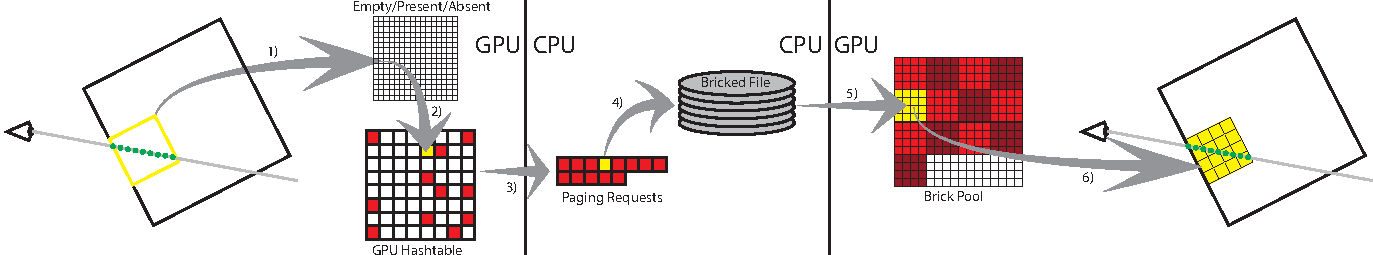
\includegraphics[width=1.00\linewidth]{images/rg/pipeline.pdf}
  \caption{The missing brick reporting / paging subsystem of our volume
  rendering approach.  Missing bricks are recorded into a hash table
  (1, 2), to be paged in (3, 4, 5) and rendered in subsequent frames
  (6).}
  \label{figrg:flow}
\end{figure*}

\section{Related Work}

Volume visualization on consumer graphics hardware has become widely
utilized as a means to cope with the growing sizes of data.  GPUs have
proven useful in both ray-tracing and rasterization
techniques~\cite{Reichl:2012:HybridSurface, Dick:2009:Terrain},
rendering of diverse scenes~\cite{Parker:2010:Optix}, as well
as considerably more general tasks~\cite{Owens:2007:GPGPU}.

Volume rendering accelerated by GPU hardware was established in the
mid-90's~\cite{Cullip:1993:AVRW, Cabral:1994:AVRA}, initially based on
hardware compositing of volume slices.  The ability to do raycasting
came later~\cite{Krueger:2003:ATGV}.  Since the time of the initial
GPU-based volume renderers, researchers have been concerned with
methods to work around the limited memory available on GPUs.  The
prominent technique for volume rendering large data on a GPU is to use
a multiresolution
representation~\cite{Boada:2001:Multires, LaMar:2000:Multires,
Weiler:2000:LoD}.  This method hinges on the concepts of empty space
leaping and early ray termination~\cite{Levoy:EarlyTermination}, two
techniques developed early on that demonstrate that sampling can be
significantly reduced in many instances of volume rendering.

There has been much work on accelerating ray-traced volume rendering in
recent years.  Voreen implements a more general architecture,
including GPU-based raycasting~\cite{Voreen:2009}.  Tuvok implements a
flexible volume rendering system with support for very large
datasets~\cite{Fogal:2010:Tuvok, Fogal:2009:SizeMatters}.  Knoll et al.
utilize a bounding volume hierarchy and optimized SSE to achieve very
fast
volume renderings~\cite{Knoll:2010:BVH}.  Gobbetti et al. and Boada et
al. detail methods for traversing tree structures on the GPU for
the purpose of volume rendering~\cite{Gobbetti:2008:VR,
Boada:2001:Octree}.
The Gigavoxels~\cite{Crassin:2009:Gigavoxels} system traverses
$N^3$-trees on the GPU to choose an effective resolution.  With the
large gap between processing power and data sizes, some communities
have turned to distributed memory systems for large-scale
volume rendering~\cite{Childs:2006:ScalableVR, Howison:2010:MPIHybrid,
Fogal:2010:HPG, Beyer:2012:DSM}.

Our algorithm employs a lock-free data structure on the GPU for
feedback information.  Highly-concurrent Lock-free structures are ideal
for the manycore GPU environment, however they have previously been
challenged by the lack of concurrency primitives available for the
OpenGL platform.  We make use of a lock-free hash table very similar to
that of Michael's~\cite{Michael:2002:LockFreeHT}, implemented in a
manner similar to Lux and Fr\"ohlich's implementation for terrain
rendering~\cite{Lux:2011:RCHeight}.

Hadwiger et al. presented a volume renderer similar to
ours~\cite{Hadwiger:2012:Guided}.  Their system is aimed at volume
rendering highly anisotropic data as it is streamed real-time from a
high-resolution microscope.  Our renderer improves upon theirs in a
number of ways:

\begin{itemize}
  \itemsep0em
  \item We perform brick lookup each brick, instead of every sample,
  maintaining the simple and familiar ray-marching core that is
  well-documented in volume rendering literature.

  \item We expound on how to use modern GPU features to implement our
  lock-free feedback data structure.  This enables the implementation
  to spend more time computing on the GPU and less time pushing data
  around.

  \item We utilize an out-of-core, progressive rendering methodology,
  breaking the GPU-memory-size barrier that limits data sizes from
  Hadwiger et al.'s work.  This also allows us to gracefully scale down
  to consumer-level graphics cards.
\end{itemize}

While we believe these to be novel additions, we do not consider them
to be this work's major contribution.  Rather, we provide new depth to
the discussions of a variety of parameters that are relevant in the
development of a ray-guided direct volume renderer:

\begin{itemize}
  \itemsep0em
  \item The strategy to be used to load higher resolution data when a
  variety of intermediate choices are possible;

  \item an understanding of the miasma of issues surrounding bricking
  and brick sizes;

  \item empirical evidence demonstrating that the working set for
  direct volume rendering is indeed bound more by the screen resolution
  than the dataset;

  \item a novel method for ray-guidance storage and propagation to the
  input system's logic;

  \item how to effectively handle real-time updates to the transfer
  function; and

  \item the effect of brick layout strategies on large volume access
  times.

\end{itemize}

% improvements upon gigavoxels:
%  . we don't require a hierarchy (but of course one can be used)
%  . they use MRTs to store their information on which brick is
%    needed.  this (a) wastes their MRTs, of which one only has 8
%    on modern GPUs, and (b) means that their memory for doing
%    this is extremely limited.  since we use image_load_store,
%    our HT for storing this is decoupled from the actual
%    rendering, and can scale up (or down) arbitrarily

In contrast to previous renderers, ray-guided volume renderers couple
the rendering process with the identification of which subvolumes
(`bricks') must be loaded.  We describe the operation of ray-guided
volume renderers, in Section~\ref{sec:algorithm}.
In Section~\ref{sec:performance} we detail a plethora of benchmarks
that demonstrate the performance of the renderer.

In many prior volume renderer evaluations, results are generally
limited to the raw performance of the renderer.  However, we note
that---for some reason---users of our volume renderer rarely ask how
many milliseconds it takes
to render the visual human.  One thing users \emph{do} ask is how large
the data can get before the renderer becomes unusable. For this reason,
we have engineered our renderer so that it does not require that the
volume fit in core.  Furthermore, users generally value a responsive
system over a performant system.  They are curious if money should be
spent upgrading a video card or buying a solid state drive.  Design
elements are carefully expounded and conclusions are drawn in
Section~\ref{sec:tradeoffs}.

Finally, Section~\ref{sec:conclusion} gives our final remarks, and note
both limitations and opportunities for future work.

\section{Ray-Guided Grid Leaping}
\label{sec:algorithm}

At the macro level, our algorithm is reminiscent of the recent work of
Hadwiger et
al.~\cite{Hadwiger:2012:Guided}, as well as Engel's
CERA-TVR~\cite{Engel:2012:CERA} that is in turn based on the Gigavoxels
system~\cite{Crassin:2009:Gigavoxels}.

With Hadwiger et al. we share the requirement of a set of simple
multiresolution Cartesian grids, along with an OpenGL-based table
to report missing bricks.  A multiresolution hierarchy is built as a
preprocess for input data that exist at only one resolution (details
are in Section~\ref{sec:tradeoffs}).  From the CERA-TVR system
we inherit the idea to only recompute and request grid cells at
boundaries.

\subsection{Overview}

We endeavor to create a volume renderer that can render massive 
datasets extremely fast on commodity GPU hardware.  The major issues in
such a renderer are:
\begin{enumerate}
  \itemsep0em
  \item Identifying regions that must be sampled densely.

  \item Precisely locating the transition between these regions and
  regions that exhibit considerable homogeneity.

  \item Terminating a ray as soon as possible.

  \item Efficiently communicating regions to be rendered in the future
  to the IO layer.

\end{enumerate}

Points (1) and (2) ensure we concentrate the computational effort on
the areas that require it.  Point (3) is critical because it means we
do not have to load the data beyond the point of early termination,
significantly reducing costly disk traffic.  If point (4) is not
sufficiently addressed, the renderer will load large amounts of data
that are not needed for rendering, at severe costs in performance.

% new subsection header here? we are switching from properties a
% Ray-guided VR needs to how we implemented said properties, here

To the first point, we employ an efficient metadata structure that
allows us to quickly identify these regions.  Points (2) and (3) are
handled through an educated choice of brick size, which is discussed
more thoroughly in Section~\ref{sec:tradeoffs}.  A major component to
modern volume renderers is how they address point (4), now by and large
based on \emph{ray guidance}.  That is, the sampling characteristics of
the ray determine which data to load.  Stated differently, the future
data requirements are computed \emph{in concert} with standard ray
traversal and accumulation.

% \todo{here we might want to say something about how regular disk I/O
% is in modern volume renderers, and allude to a later section where we
% discuss data organization}

The entire operation is detailed in Figure \ref{figrg:flow}. For each
ray we compute the level of detail required to maintain a pixel error
of less than one. With this level and the position in the volume we
compute a brick index.  This brick index is used to fetch information
from a lookup table
(Figure \ref{figrg:flow}.1) to identify whether the brick is a) empty, b)
non-empty and present on the GPU, or c) non-empty and absent. When it
is empty, we skip the brick and repeat the process at the brick's exit
point.  When it is non-empty and present, we ray-cast that brick. When
the brick is non-empty \emph{and} not resident in GPU memory, the
system returns the finest coarser level available and the missing entry
is added to a GPU hash table (Figure
\ref{figrg:flow}.2). This table is read back to the host memory at the
end of the frame (Figure \ref{figrg:flow}.3), and used to page in bricks
from
disk or cache (Figure \ref{figrg:flow}.4).  A paged-in brick is then
uploaded to a GPU texture pool
(Figure \ref{figrg:flow}.5), and a subsequent frame will use this
portion of the brick pool for sampling (Figure \ref{figrg:flow}.6).

% While we do not require a full hierarchy---only that coarser versions
% of the data exist---we generate a multiresolution hierarchy for such
% data as a preprocess.

The key component is that both ray-accumulation \emph{as well
as} identification of the bricks that are needed should occur
on the GPU.  The latter is natural to compute during standard
ray-casting operations.  Doing both operations on the GPU means brick
identification comes very cheap, as it parallelizes very effectively.
More importantly, performing this during ray-casting ensures that it
is optimally accurate: the program never loads data that will not be
used.

%---we get results which are as accurate as the brick size.

\begin{algorithm}
  \caption{Ray-guided volume rendering.  Each ray identifies the
  set of bricks that it needs for rendering independently, and
  reports this information for use in subsequent rendering passes.}
  \label{alg:vrender}
  \begin{algorithmic}[1]
%  \If{$rayResumePos = FINISHED$} \Return \EndIf
  \State \textit{color} = \textit{rayResumeColor}
  \State \textit{terminated} = \textbf{true} \Comment{assume ray will finish}
  \State \textit{rayResumePos} = \textbf{FINISHED}
  \Repeat
    \State \textit{LoD} = ComputeLOD(Depth(\textit{ray}))
    \State \textit{brick, samplingRate} = GetBrick(\textit{ray})
    \State \textit{offsets} = PoolOffsets(\textit{brick})
    \If{\textit{samplingRate} $\neq$ RequiredSamplingForLOD(\textit{LoD})}
      \State ReportMissingBrick(\textit{brick})
      \If{\textit{terminated}} \Comment{\emph{first} missing brick?}
        \State \textit{terminated} = \textbf{false}
        \State \textit{rayResumePos} = \textit{ray}
      \EndIf
    \EndIf
    \State Raycast(\textit{ray}, \textit{samplingRate}, \textit{offsets})
  \Until{\textit{ray} $\geq$ \textit{exit} $\lor$ Saturated(\textit{ray})}
  \State \textit{rayResumeColor} = \textit{color}
  \end{algorithmic}
\end{algorithm}

The basic algorithm is given in Algorithm \ref{alg:vrender}.  Briefly, the
appropriate sampling rate is identified and we look for the data at
that resolution (lines 6, 7).
\texttt{GetBrick} will always return some data, but the data may be at
a lower resolution than request; this is
communicated through the \texttt{samplingRate} and the situation is handled
on line 8.  If our data are too coarse, we note that we are missing a
brick (\texttt{ReportMissingBrick}) and where we are in the volume
(\texttt{rayResumePos}) when
this \emph{first} occurred (\texttt{terminated}).

% A key insight is that the relationship between \texttt{GetBrick} and
% multiresolution data can be entirely opaque.  The function simply
% takes a region and returns a chunk of memory to be ray-traced, with
% information as to how it should be sampled.  In contrast to the
% Gigavoxels system, a strict hierarchy is not required, and indeed our
% system does not organize data on the GPU in this manner.

% \begin{algorithm}
%   \caption{Ray-casting inner loop.  Operation is equivalent to a
%   traditional ray-casting volume renderer, with the minor addition
%   of offsets into the volume pool.  Checking in the outer loop is
%   sufficient and allows this core inner loop to stay simple.}
%   \label{alg:inner-loop}
%   \begin{algorithmic}[0]
%     \While{$ray \not\geq$ Exit($brick$)}
%       \State $v =$ sampleVol($ray$ + $offsets_{pool}$)
%       \State $c =$ TransferFunction($v$)
%       \State $color = color + (1 - \alpha) \times c$
%       \State $ray = ray + stepSize$
%     \EndWhile
%   \end{algorithmic}
% \end{algorithm}

Every iteration through the outer loop, we perform this identification
of the appropriate resolution.  This satisfies our first goal as
mentioned above: we identify the appropriate sampling resolution
at every brick boundary.  With small bricks, this means we will do
few integration steps before early ray termination is recognized.
Furthermore, we detect empty bricks at this stage as well.  The
standard
raycasting inner loop is hidden in the \texttt{Raycast} call.

% The \texttt{Raycast} function is listed in Algorithm
% \ref{alg:inner-loop}.  Note that this is equivalent to `standard'
% ray-casted volume rendering in more traditional volume renderers,
% sans the minor addition of \texttt{offsets} when sampling the
% volume data.  In fact, this is not a unique aspect of our renderer;
% any renderer which uses a volume pool would share this code.  The
% simplicity of the volume rendering loop is a prime benefit to our
% approach; the entire GLSL core consists of less than 600 lines of code,
% including all the debugging and profiling targets used to generate
% images and timing results for this paper.

% \subsection{Mixed Levels of Detail}
% 
% As the sampled resolution can differ at arbitrary points along the ray,
% a natural concern is what sampling methodology is required to ensure
% these boundaries are not visible in the rendering.  In this section, we
% demonstrate empirically that no advanced sampling schemes are required.
% 
% The appropriate sampling rate for a given region of space is a function
% of the frustum settings and the depth of the current sampling position.
% The depth is the only parameter which varies
% \emph{while} we progress along a ray.  Moreover, the appropriate
% sampling rate is aliased to the relatively few levels of detail which
% are available for a dataset.
% 
% \begin{figure}
%   \centering
%   \includegraphics[width=\linewidth]{images/simultaneousLoDs-1}
%   \caption{Volume rendering of the full color visible human dataset
%   with color-coded levels of detail.  It is difficult to derive viewing
%   conditions for which a plethora of LoDs are required; the relatively
%   few LoDs visible here come from an extreme case.}
%   \label{figrg:LODs}
% \end{figure}
% 
% In practice, even for highly anisotropic data, it is difficult to
% derive frustum and viewing angles which result in the simultaneous
% visibility of more than three levels of detail.  Figure
% \ref{figrg:LODs} demonstrates this: as the ray switches from one level
% of detail to another, the color is flipped---bricks rendered at the
% highest resolution for the viewpoint are in red, and the lowest
% resolution data has a blue tint.  Looking at these areas side-by-side,
% it is clear that such boundaries are not visible in normal volume
% renderings.
 
%% this was moved to a single sentence at the beginning of sec:algorithm
% \todo{This paragraph feels really out of place here, but we need something
% similar \emph{somewhere} (reviewer comment)} Of course, many volume
% datasets are not provided in a multiresolution form.  For such data,
% we generate multiresolution representations as a preprocess.  This need
% only be done once, of course, and is relatively fast: 72 minutes on
% a modern Intel i7 machine for a typical case, the Richtmyer-Meshkov
% instability (`RMI', $2048x2048x1920$ voxels).  We note, however, that
% this process scales very poorly with the brick size: small brick sizes
% take considerably more time. More
% discussion is provided in Section~\ref{sec:tradeoffs}.

% or 5391.92 seconds / 60 = 89.87 minutes on a Xeon

\subsection{Missing Data}

As noted above, it is possible that data are undersampled while
rendering.  When this occurs, we display a coarser version of the data
initially, but progressively refine those regions with finer resolution
data until they are sampled at a rate of a single voxel per pixel, or
the maximum data resolution available.  This information is collected
by the GPU as it renders, but must be communicated back to the CPU to
coordinate disk access and update the appropriate area of the volume
pool.

One solution for this would be to use multiple render targets to store
information on which bricks are missing~\cite{Crassin:2009:Gigavoxels}.
The limitation of this method is the limited mapping operation from
the ray to the target buffer: there are only so many available render
targets.
Furthermore, this approach ignores the inherent spatial coherency
between rays.  Two neighboring rays are highly likely to request the
same set of bricks, or at least have substantial overlap within the
sets they require.  With the multiple render targets approach, both
pixels will encode the same value, and we will need to read back larger
textures that consist of predominantly duplicate values.

Instead of utilizing extra render targets, we take advantage of an
OpenGL extension that was promoted to core in version 4.2,
\texttt{GL\_ARB\_shader\_image\_load\_store}.  This extension allows
the creation of an image buffer that is independent of the current
rendering buffer.  Using the atomic load/store operations the extension
provides, we implement a set based on a linearly-probed lock-free hash
table stored in an \texttt{image\_load\_store} buffer.  Since we are
hashing based on the brick, multiple rays requesting the same brick hash
to the same position.  This allows us to keep the table---and therefore
how much information we read back per-frame---quite small.  We discuss
sizing of the hash table in more detail in
Section \ref{sec:ht-params}.

\begin{figure}[t]
  \centering
  \includegraphics[width=0.95\linewidth]{images/rg/terminate-empty.png}
  \caption{Volume rendering behavior for the Mandelbulb dataset.
  Green indicates bricks that were skipped via empty space skipping.
  Red indicates bricks that were sampled densely.  Blue indicates
  bricks that were sampled but saturated quickly.
%  Most rays skip almost all of the data or terminate very quickly;
%  the lack of white regions in this rendering indicate that, here,
%  \emph{all} rays fall into a single category.
  }
  \label{figrg:bricks-empty}
\end{figure}

\begin{figure*}
  \centering
  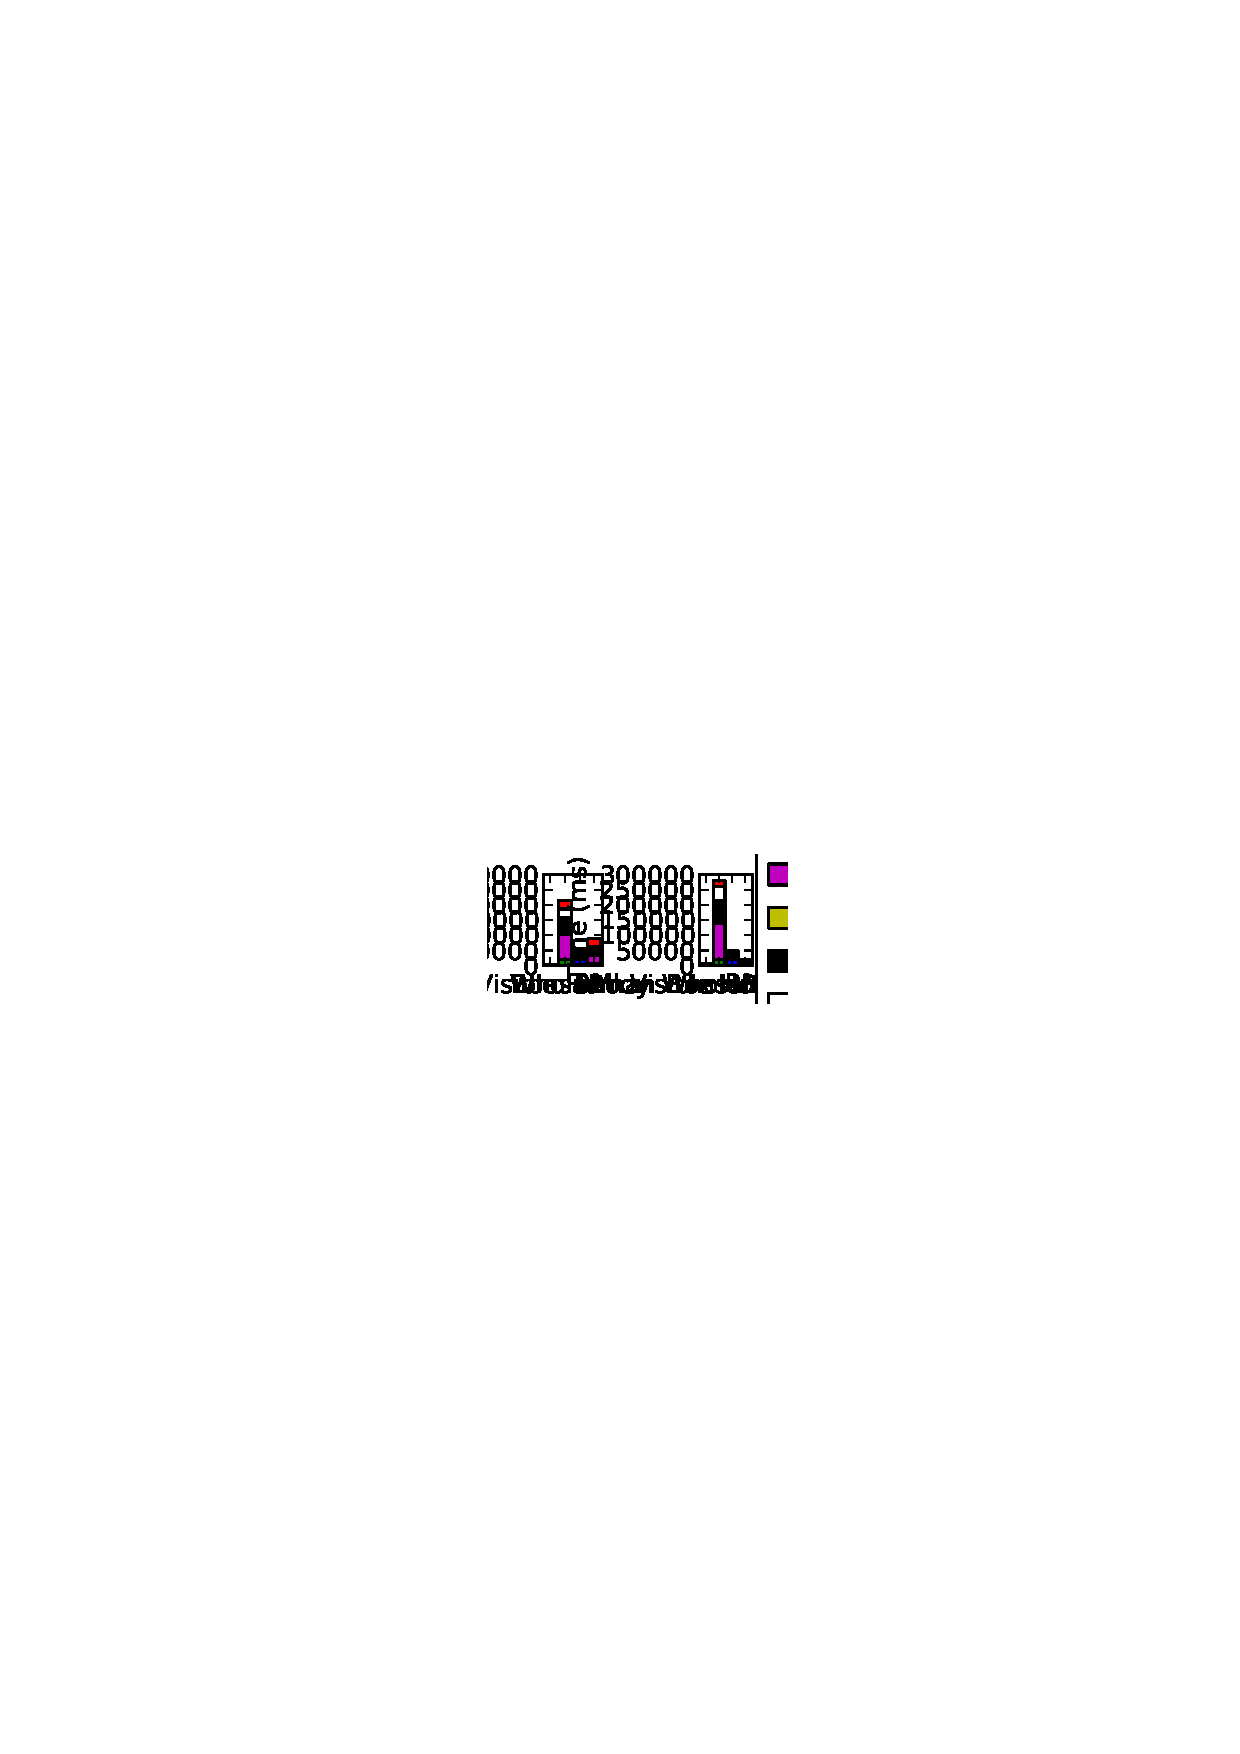
\includegraphics[width=1.00\linewidth]{images/rg/breakdown.pdf}

  \caption{Time spent at various stages of our pipeline, aggregated
  over the generation of a rotation sequence.  Comparisons are made
  between data stored with the ideal brick size for that dataset
  (`Native'), and data stored at a large brick size of $256^3$ with
  the ideally-sized bricks created at run-time (`Rebricked').  `Whole
  Body', `Velocity', and `Magnitude' suffer from a lack of ray
  saturation.}

  \label{figrg:breakdown}
\end{figure*}

\subsection{Brick Classification}
\label{sec:brick-classification}

Considering our target goals (1) through (3) given at the beginning of
this section, one could classify a brick into one of three categories:
\begin{itemize}
  \itemsep0em
  \item skipped due to empty space skipping,

  \item early termination due to ray saturation, or

  \item sampled densely without saturating.
\end{itemize}

An important observation is that---in a very large number of
cases---bricks fall into \emph{either} the `empty' or `saturating'
categories, and only \emph{rarely} in the `non-saturating' category.
The factor that has the greatest effect on performance is how quickly
a renderer can classify data into one of the first two categories, and
therefore bypass a large set of the work.

To make this identification effective, ray-guided volume renderers
maintain the state of each brick, shared on both the GPU and host
memories.  During rendering, one uses the table to identify if a brick
is empty.  If so, the renderer leaps over that space instead.  We store
this as an array consisting of one 32-bit integer per brick of the
dataset.

Figure \ref{figrg:bricks-empty} visualizes this classification for a
large dataset under a typical view and transfer function.  As shown
there, the majority of the visualization falls into either the `blue'
(saturated quickly) or `green' (skipped) sets. This also demonstrates
how little data is actually required for a typical volume rendering.  A
similar rendering is given in the rightmost image of
Figure~\ref{figrg:teaser}, in which only the rays in the middle of the
volume require high computation.

Of course, this classification depends largely on the transfer function
and viewing parameters.  In practice, however, transfer functions that
produce \emph{informative} visualizations tend to exhibit such ternary
classifications.

When the transfer function is changed, this metadata information
must be recomputed.  For datasets with many bricks, this can induce
a noticeable delay.  Our current test platform can process about
7.5 million bricks per second, but even a 1 second delay between
interactions is too much.  Therefore, we offload this update to a
background thread.  Until the thread completes its work, the renderer
considers all unprocessed bricks to be `missing', causing it to request
bricks that might be empty.  Those bricks' metadata are directly
updated and they are only loaded if they fail the empty check.  The
overall performance effects may be large, but the system remains
responsive during this period.

\section{Performance}
\label{sec:performance}

In this section, we give an overview of the various stages of the
renderer and how they perform.  Unless otherwise noted, all timings
were performed on a dual quad-core Xeon 2.2~GHz system using an NVIDIA
GeForce GTX 680, with 24~GB of system memory and 4~GB of GPU memory.
We mostly report results from commodity hard drives, explicitly noting
some specific relevant uses of SSDs.  In many cases, results were
obtained from multiple screen resolutions, but we report results from
an HD viewport ($1920\times1080$) unless noted otherwise.  Details of
the data utilized and renderer timings are given in
Appendix~\ref{sec:data}.

\subsection{Benchmarks}

We have chosen a variety of benchmarks to evaluate the performance of
our renderer, and we elucidate the logic behind those choices here.
First, the choice of HD resolution is motivated by voxel-to-pixel error
ratios.  All modern high-performance volume renderers try to maintain a
1-to-1 ratio between projected voxels and pixels.  Adaptive resolution
selection is used to ensure this ratio.  Without this feature, results
will be aliased, too much information will be compressed to a single
pixel, and performance will suffer.  Adaptive resolution means that
small viewports will not stress renderers: a 512$\times$512 viewport
can get along fine with a paltry few hundred megabytes of memory,
irrespective of the input dataset size.

We utilize zoom-ins, as in the accompanying video and results such as
those in Figure~\ref{figrg:working-set} and some in
Table~\ref{tbl:timings}, to accentuate these high resolution issues.
When the volume is far away, a very coarse resolution is utilized that
maintains accurate voxel-to-pixel error ratios.  As the camera comes
closer, higher resolutions of the source data must be utilized.  We
terminate zoom-ins slightly after they fill the screen; beyond this
point, frustum culling's effect dominates (see
Figure~\ref{figrg:working-set}).  The most challenging cases for a
volume renderer are when data are close enough to be seen at native
resolution, but far enough away that no data can be culled by the
frustum.

Rotations are used to demonstrate that the renderer does not rely
solely on early ray termination.  As described in
Section~\ref{sec:brick-classification} and depicted in
Figure~\ref{figrg:bricks-empty}, most rays either skip large parts of
the volume, or terminate very quickly.  With a transfer function that
produces a dense volume, bricks in the front will prevent bricks in the
rear from ever being paged in, effectively meaning the volume renderer
need only cope with the front \emph{half} or even less of the volume.
Barring pathological volumes and transfer function choices, rotations
ensure all of the data has a chance to contribute to a sequence.

\paragraph{Transfer functions.} Changing a transfer function is also
an important benchmark in any volume rendering system.  Doing so
invalidates our brick metadata concerning which bricks are empty,
causing some hash table entries in the next frame to make little sense
(i.e. request bricks that are visible under the old transfer function
but empty under the new one).  Furthermore, the bricks in the GPU
volume pool may be inappropriate for the new transfer function.

Renderer performance as measured by response time during such an
interaction actually changes very little, and can even improve.
However, quality suffers rather drastically.  This is evident in the
time to convergence after a change in the transfer function: in a
typical case with the RMI data set (see Section~\ref{sec:data}), time
to convergence increased over 6x after changing the transfer function
(from $\sim$380ms to $\sim$2300ms).

\begin{figure*}
  \centering
  \includegraphics[width=0.98\linewidth]{images/rg/workingSets1-150dpi.pdf}
  \caption{Working set sizes across three different scenarios for
  multiple datasets.  Smaller brick sizes approximate the working set
  better.}
  \label{figrg:working-set}
\end{figure*}

\subsection{Results}
\label{sec:results}

To evaluate our renderer in different scenarios, we used a standard
rotation scenario with a variety of datasets, measuring the length of
each pipeline stage.  Figure~\ref{figrg:breakdown} has these results.  As
IO is the prime bottleneck in many cases, we implemented a `rebricking'
scheme to mitigate the amount of IO performed.  Using large reads and
caching, this significantly lowers the time spent doing IO.  We used
`LZ4' compression when recording this performance data, which trades
CPU time for IO time.

The majority of the time is spent ray-casting, pulling data from disk,
and uploading the bricks to the pool.  Our novel hash table approach
keeps the table small, and so reading it is very cheap: even for large
data, this component does not factor in to the overall performance.
The other GPU data to manage is metadata information for our volume
pool (i.e. which bricks are resident), but at a single machine word per
brick it costs very little to push it down to the GPU, even for very
large data.

Interestingly, the time spent managing GPU data is an increasing
function of volume size \emph{until} it peaks around the size of the
RMI ($2048\times2048\times1920$).  This reinforces our assertion that
there is only so much data visible in a given frame---dependent only on
the view
frustum, and \emph{not} the dataset size---and so at some point we
saturate the set of visible data.  Figure~\ref{figrg:working-set} and
Section~\ref{sec:subdivision} include more discussion about working set
sizes.

% \todo{datasets to beat/compare with:
% 2048x1024x1080, 16bit, 640x480 viewport: 95 minutes to preprocess
% ($32^3$). biomedical data (lizard scan?).  12 to 30 Hz range; avg 16 Hz
% for volume rendering, avg 20 Hz for
% iso. dvr had peak memory use of: 153.125 megabytes\cite{Gobbetti:2008:VR}.\\
% 21494x25790x1850, 1024x768 viewport. ``mouse cortex''. two transfer
% functions: one runs at 75 Hz, another at 12.\cite{Beyer:2012:DSM}\\
% 18000x18000x304, 1024x768 viewport.  77 Hz and 19
% Hz\cite{Beyer:2012:DSM}.\\
% $2048^3$, 1024x768 viewport.  55 and 30 Hz.\cite{Beyer:2012:DSM}.
% }

\section{Design Tradeoffs}
\label{sec:tradeoffs}

In this section, we try to explore aspects that have not been
thoroughly addressed by previous literature.  Details on trade-offs and
the reasoning behind our final implementation choices are given.

% There are a variety of considerations in a ray-guided volume renderer
% which have not been thoroughly addressed in previous literature.  We
% endeavor to explore some of these choices here, and explicitly detail
% the inherent trade-offs and reasoning behind our final decisions.

\subsection{Subdivision}
\label{sec:subdivision}

How a system subdivides the volume into manageable pieces can have
a large effect on the performance of the renderer.  The primary
considerations are in regard to early ray termination and empty space
skipping: small bricks are much more likely to be composed of a small
range or even uniform values, which will make it more likely that the
brick can be skipped under a large set of transfer functions.  Further,
small bricks means one will detect ray saturation much more quickly, as
this is checked only when exiting a brick.

\paragraph{Internal Overhead}

The primary drawback is reduced disk throughput due to utilizing many
small requests.  A further drawback is the data size overhead: each
brick needs two voxels of ghost data in each dimension, for sampling
and gradient computation purposes.  This is negligible for large
bricks, but grows sharply as the brick size approaches one, as shown in
Figure
\ref{figrg:brick-size}. Figure~\ref{figrg:hierarchy-build} demonstrates
that this is not strictly a theoretical result: a small brick size
greatly increases not just size overhead, but also the time to
reorganize the data on disk.  From these Figures we can derive that for
large datasets a brick size of less than $16^3$ is impractical.

\paragraph{External Overhead}

We have performed a number of experiments to identify the working set
size for multiple different brick sizes.  Starting with the smallest
practical size of $16^3$, we increase the brick size up to $512^3$.

As can be seen in Figure~\ref{figrg:working-set} the working set is bound
not by just the data size, but the screen resolution as well.  It can
also be seen that the brick size heavily influences the working set
size: larger bricks allow for less efficient utilization of empty
regions. From the images we can derive that a brick size of less than
$128^3$ is desirable to reduce the working set to roughly the memory
size of a GPU.

We note that the working set size is not a strict function of the brick
size, however.  Figure~\ref{figrg:working-set} and
Table~\ref{tbl:timings} also show that the choice of brick size is not
clear-cut.  The Visible Human male performs best with $16^3$ bricks,
for example, whereas the ideal brick size for the `Magnitude' data is
$64^3$.  For the `Whole Body' dataset, using brick sizes of
$16^3$ actually resulted in \emph{larger} working sets than $32^3$.
This occurs when the transfer function produces large regions
of semi-transparency but never reaches saturation.  Indeed, when datasets
contain large swaths of semi-transparent regions, the conventional
wisdom is reversed: large brick sizes are generally preferred, since
they significantly improve disk throughput.

% \paragraph{Performance}
%
% There are three primary metrics to be concerned with when evaluating
% a volume renderer's performance.  One of them is the commonly
% evaluated metric: the time required to render the data at the
% required resolution.  The second is system responsiveness: if the
% user changes a viewing parameter, a transfer function, or any other
% state, the renderer should respond quickly.  A third consideration is
% the time to generate these data: converting a large dataset into a
% bricked representation grows sharply as the brick size shrinks.
%
% \todo{table or graph of brick size (X) and `time to build hierarchy' (Y)}

%% moved this up into other paragraph
% As can be seen Table \ref{tbl:timings} and Figure
% \ref{figrg:working-set}, the brick size choice is not clear-cut.
%   The
% Visible Human male performs best with $16^3$ bricks, for example,
% whereas the ideal brick size for the `Magnitude' data is $64^3$.  When
% the transfer function keeps large regions mostly transparent, as is the
% case for the `Whole Body' and `Velocity' datasets, then the improved IO
% performance gleaned from large requests derives the most benefit.

If we begin to consider secondary metrics, such as the response time of
the system, the choice of brick size becomes even more complex.  Since
bricks are the atomic building blocks in a volume renderer, one cannot
load less than a single brick from disk. Therefore a larger brick size
imposes a larger response time on the system.  These concerns would
generally push a designer to choose smaller bricks.

However, disk performance falls very sharply with small
requests~\cite{Fogal:2011:PracticalIO}.  It is nice for a system to
respond within a few tens of milliseconds, but such concerns should not
dictate the design to the point that end-to-end performance suffers
drastically.  Furthermore, small brick sizes are accompanied with
significant
overhead, as discussed in Figure \ref{figrg:brick-size}, and do not
compress as effectively as their larger counterparts.

Systems such as Reichl et al.'s hybrid surface rendering, CERA-TVR, and
Gigavoxels utilize a static brick size of
$32^3$~\cite{Reichl:2012:HybridSurface, Engel:2012:CERA,
Crassin:2009:Gigavoxels}.  This brick size exhibits few extremes of the
performance issues mentioned above. However, it is certainly not the
ideal choice for all circumstances.

\begin{figure}
  \centering
  \includegraphics[width=0.99\linewidth]{images/rg/BS-overhead.pdf}
  \caption{Brick size overhead.  As bricks get smaller, the overhead
  for the additional ghost data grows significantly.  At a larger brick
  size of $128^3$, the overhead with 2 ghost voxels per dimension
  amounts to a few percent, whereas with $32^3$ bricks this increases
  the dataset size by almost 50\%.}
  \label{figrg:brick-size}
\end{figure}

\subsection{Disk IO}

\subsubsection{Brick Layout}

Figure~\ref{figrg:layout} demonstrates how this changes with the brick
size.  Both disk IO times as well as decompression times are displayed
there.  As shown in the figure, reading data from disk becomes quite
severe with small brick sizes.  However, as brick sizes grow to $64^3$
and beyond, decompression time becomes more important and overall time
plummets.  This effect is even more pronounced using a hard disk in
place of the SSD used here.  Intelligent layout strategies purport to
minimize seek times; our results corroborate this, with the important
caveat that seek times are not relevant with larger brick sizes.

\begin{figure}[tb]
  \centering
  \includegraphics[width=1.00\linewidth]{images/rg/brickIO-RichtmyerMeshkov-ZoomIn-SSD.pdf}

  \caption{Time spent with IO-related tasks using an SSD for the
  RMI dataset's zoom-in scenario, sampled with 100 frames and a
  $1024\times768$ viewport.  Layout strategies only see utility at
  small brick sizes.}

  \label{figrg:layout}
\end{figure}

% \begin{figure}
%   \centering
%   \includegraphics[width=\linewidth]{images/dsize-rtime}
%   \caption{\todo{needs update, data is made up (alex: benchmark! run
%   dsize-performance.lua)} Total rendering time, including brick IO,
%   to generate animations for the `mandelbulb' dataset at various
%   sizes and two distinct layouts.  Brick size was $32^3$ for all
%   runs.  Layout scheme has relatively little impact: disk read time is
%   negligible relative to the entire process.}
%   \label{figrg:rtime-layout}
% \end{figure}

\subsubsection{Dynamic Rebricking}
\label{sec:rebricking}

% \todo{this is too long. important message: rebricking is a good idea,
% because it avoids absurd hierarchy build times and gives good I/O
% performance. the overhead is demonstrably minor.}

The renderer desires small bricks, as discussed in
Section~\ref{sec:subdivision}, as small bricks will help with early ray
termination and empty space leaping.  However Figures~\ref{figrg:layout}
and \ref{figrg:brick-size} clearly demonstrate that large brick sizes
are preferable for disk performance and overhead reasons.  To provide
the best of both worlds, we implemented a `dynamic' bricking scheme,
whereby bricks are stored on disk in a rather large size (e.g. $256^3$)
but presented to the renderer as if they exist at some small resolution
($32^3$).  The small bricks are dynamically generated from the large ones on
request.

Since requesting a large brick for every small brick would only
increase the disk traffic, we keep an additional brick cache in memory
to source these copies from.  Our cache uses a standard LRU strategy.
This is advantageous when the working set of the data fits into the
host memory, however when the working set exceeds the host memory we
will evict entries before finishing a rendering.  We stuck with this
strategy since the working set
often \emph{does} fit into host memory, as established by
Figure~\ref{figrg:working-set}.  If the renderer is to be used in an
environment in which working sets are routinely larger than memory, an
MRU strategy would be more appropriate.

\paragraph{Hierarchy Generation}

Reorganizing data into a set of bricks is mostly ignored in volume
rendering literature, but becomes a significant bottleneck in
real-world usage.
Figure~\ref{figrg:hierarchy-build} shows the time our preprocess needs
to generate this hierarchy, which increases sharply for small brick
sizes.  This time also increases with respect to dataset size.  At
the extreme scale, such data reorganization is completely infeasible:
merely reading every datum might take months.  We believe such
reorganization will be feasible up to a few tens of terabytes.  In
practice, the authors and collaborators thereof tolerate this for up to
5 terabytes at present.

% For the case of visualization-based verification, a dataset might
% only need to be loaded once to identify that a parameter was set
% wrong; this data reorganization is then a very high cost to pay.

Rebricking the data at run time alleviates this problem.  The data can
be generated at very large brick sizes, enabling fast conversion and
effective disk throughput, and then dynamically rebricked to very small
sizes.  Both disk and renderer deal with their ideal cases, then.  The
`Rebricking' case of Figure~\ref{figrg:breakdown} shows performance in
this mode.

%% compression isn't unique enough to have its own story, particularly
%% since we need space.

% \subsubsection{Compression}
% 
% Regular gridded data typically contains large areas of uniform
% values.  One example is in the outer regions: most scanners as well as
% simulation software produce many layers of zeroes outside the region of
% interest.  Especially in simulation output, there may be large areas in
% a dataset which change at a very low frequency, producing runs of the
% same data value. All of these regions compress very effectively.
% 
% \todo{make it clear we are compressing each brick in isolation, storing
% it compressed on disk, and decompressing it when it is read---before it
% makes it to the renderer}
%
% \begin{figure}
%   \centering
%   \includegraphics[width=\linewidth]{images/Compression}
%   \caption{Compression ratios for a variety of datasets using the
%   `fastest' zlib compression mode.  Very often, data compress to a
%   factor of less than half their original size. \todo{Alex will replace
%   this graph}}
%   \label{figrg:compression}
% \end{figure}
%
% \todo{Need results for (\emph{many}!) more datasets!}

% The zlib libary has given us very good results for many datasets.
% Some results on the compression ratio are given in Figure
% \ref{figrg:compression}.  Our system compresses data per-brick, and is
% instrumented to keep track of the data sizes both before and after
% compression.  Interestingly, these brick sizes \emph{always} shrink:
% we have not identified a single brick in any depicted (as well as many
% other) datasets for which the post-compression size is increased.  We
% attribute this to the addition of ghost data, which enlarges even the
% smallest brick to $3^3$.

\begin{figure}[tb]
  \centering
  \includegraphics[width=0.98\linewidth]{images/rg/HierarchyBuildTime.pdf}
  \caption{Time to build bricked representation for a medium-sized dataset,
  as a function of brick size.  Renderers desire small bricks to
  perform efficiently, but generating such bricks takes significant
  preprocessing resources.}
  \label{figrg:hierarchy-build}
\end{figure}


\begin{figure*}
  \centering
 \begin{minipage}[t]{0.3651225\linewidth}
   \begin{algorithm}[H]
   \caption{Greedy algorithm: request all bricks at all
   resolutions.\vspace{0.1em}}
     \begin{algorithmic}[H]
     \State ReportMissingBrick(\textit{b}) \Repeat
       \State \textit{LoD++}
       \State \textit{b} = LookupBrick(\textit{ray}, \textit{LoD})
       \If{Missing(\textit{b})}
         \State ReportMissingBrick($b$)
       \EndIf
     \Until{$\lnot$Missing(\textit{b})}\\
     \end{algorithmic}
   \end{algorithm}
 \end{minipage}
 \hfill
 \begin{minipage}[t]{0.55\linewidth}
   \begin{algorithm}[H]
   \caption{Global algorithm: only request bricks required to satisfy
   the final rendering request.\vspace{0.000em}}
     \begin{algorithmic}[0]
       \State ReportMissingBrick(\textit{b})
       \Repeat
         \State \textit{LoD++}
         \State \textit{b} = LookupBrick(\textit{ray}, \textit{LoD})
       \Until{$\lnot$Missing(\textit{b})}
     \end{algorithmic}
   \end{algorithm}
 \end{minipage}

  \includegraphics[width=\linewidth]{images/rg/strategy.png}
%   \includegraphics[width=0.99\linewidth]{images/Algorithm-Global}
%   \includegraphics[width=0.99\linewidth]{images/Algorithm-Greedy}
  \caption{The effect of multiple brick replacement strategies.
  Renderings are select intermediate frames from the corresponding
  strategy.  `Greedy' strategies converge quicker and produce more
  densely-packed intermediate progress.}

  \label{figrg:strategy}
\end{figure*}

\subsection{CPU/GPU Interface}

Point (4) in our overview is the efficient communication of the ray
guidance information from the location it is generated---the GPU---to
the location it is utilized---the IO layer of a volume renderer.  This
section details how that communication happens.

We utilize a GPU-based hash table to store this data, though we note
that we really only require a set.  That is, our keys (brick IDs) are
our values, and we only care about their \emph{presence} in the table,
which we will read back and process as a list later.  A list would work
as well, but a hashing scheme allows concurrent inserts to proceed with
less contention.  During rendering, a ray may write into this table to
indicate that it
needs a non-resident brick to continue (see Figure \ref{figrg:flow},
(c)).  This small table will be read back from the GPU at the end of a
frame and utilized to fill the volume pool with new data.

As locks do not exist in current GLSL versions (and potentially never
will), lock-free structures are the only hazard-prone data structures
that can be correctly implemented.  Crassin et
al.\cite{Crassin:2009:Gigavoxels} workaround this by using multiple
render targets: each pixel has its own unique set of memory to
write into, and so there are no write hazards.  Our scheme requires
significantly less memory, but we must deal with these write hazards.

\subsubsection{Hash Table Parameters}
\label{sec:ht-params}

We map from the 4D index of the requested brick (spatial index + LoD)
to a unique 1D index in the hash table.  The mapping we utilize is
simply converting the 4D index into its equivalent 1D form, as if it
were stored in a 1D array.  We increment the index by 1 so that we may
use 0 to indicate that there is no entry at a location.

In a normal concurrent hash table, a lock is acquired for a table or
bucket before an access.  In lock-free data structures the primitives
used to implement locks are instead used directly on the data values
in question.  Inserts into our table proceed mostly as described in
previous
work~\cite{Michael:2002:LockFreeHT}.  In the face of concurrent
writes, this operation fails, and we attempt to probe a few times
(presently: 10) before giving up.

The critical piece to note is: \emph{it is not an error if a
missing brick is not recorded}.  As long as \emph{some}
missing bricks are recorded, the next frame \emph{will} make progress.
Each ray is either: finished, able to make progress, or unable to make
progress due to a lack of bricks that it requires.  Since our hash
table only contains entries for bricks that were requested by a ray,
then an invariant of our system is that: volume rendering is done, or
there exists at least one ray that can make progress.

% When a large number of bricks are needed, the hash table fills
% consistently, implying that collisions are infrequent or unimportant.
% If we vary the number of times rehashing is attempted from 5 to 100,
% for example, then performance differs by less than sampling noise,
% and the number of subframes decreases by barely 5\%, suggesting that
% collisions happen infrequently.

% Intuitively, the hash table size would have a large effect on
% performance.  Large tables should enable recording \emph{every}
% missing brick in a single pass, reducing the number of total passes
% required before convergence.  However, we found the size parameter
% to be negligible.  Regardless of how many rendering passes one does,
% the overall work is the same: the number of rendering passes will not
% change the number of bricks which must be loaded and rendered.  The
% only additional cost to an extra pass is the per-frame setup, which
% is independent of data size.
%
% One effect that small hash tables \emph{do} have is that they improve
% the response time of the renderer.  Since the next frame cannot begin
% until all bricks in the hash table are loaded, a small hash table
% creates a more iterative, progressive rendering experience.

\subsubsection{Strategies for Loading Coarser Bricks}

When the resolution required is missing during ray-casting, a ray's
brick requests can be what we call `greedy' or `global'.  In the
`greedy' case, the ray requests intermediate levels of detail along the
way, flooding the hash table with
requests that \textit{this} ray wants.  In the `global' case, each
ray only requests what it absolutely needs, leaving space for other
rays to request what they need.  These cases are visually depicted and
expounded in Figure
\ref{figrg:strategy}.

% \begin{figure}
%   \centering
%   \includegraphics[width=0.99\linewidth]{images/Algorithm-Global}
%   \caption{The effect of multiple brick replacement strategies.
%   Renderings are select intermediate frames from the corresponding
%   strategy.  `Greedy' strategies converge quicker and produce more
%   densely-packed intermediate progress.}

%   \label{figrg:strategyGlobal}
% \end{figure}

% \begin{figure}
%   \centering
%   \includegraphics[width=0.99\linewidth]{images/Algorithm-Greedy}
%   \caption{The effect of multiple brick replacement strategies.
%   Renderings are select intermediate frames from the corresponding
%   strategy.  `Greedy' strategies converge quicker and produce more
%   densely-packed intermediate progress.}

%   \label{figrg:strategyGreedy}
% \end{figure}

The intuitive interpretation is that the `greedy' approach will produce
a more responsive, iteratively-refined image, whereas the `global'
approach will generate the final correct image quickest.  However, the
authors were surprised to find that the `greedy' approach both produces
more pleasing progress information \emph{and} converges in the fewest
number of frames.  This is because it allows a ray to sample at its
final resolution quickly, which can cause earlier ray termination.

\section{Conclusions, Limitations, \& Future Work}
\label{sec:conclusion}

In this work, we have introduced an efficient, out-of-core, ray guided
GPU volume renderer that scales to extremely large data.  The system
pulls inspiration from a patchwork of recent renderers, combining the
advantages of many and reimplementing some ideas in light of modern GPU
features.  We have also contributed an evaluation and discussion of the
tradeoffs inherent in the development of a modern ray-guided volume
renderer.

Based on the data here, we conclude that a ray-guided volume renderer
should work with bricks that are, on disk, $64^3$ or larger.  This
minimizes time spent doing IO (Figure~\ref{figrg:layout}), and makes
data layout irrelevant, obviating the need for a complicated component
of the code.  Since the required memory shrinks with the brick size,
generating $32^3$ or even $16^3$ bricks on-the-fly is desirable,
though exactly which size is unfortunately too data-specific to answer
generally.  While `bzlib' gives ideal compression ratios, it is very
slow to decompress, and therefore most implementations will want to
utilize `LZ4' compression.  A cache is a boon when data will not fit in
GPU memory but will fit in the host's memory.

We have made a best-effort attempt to design both favorable and
unfavorable conditions with which to test a volume renderer, but it
is possible some considerations have been omitted.  In particular,
this renderer and many others rely heavily on the assumption that
rays will saturate quickly.  Subjectively, we have found this to be
overwhelmingly valid for all our work in volume rendering, but this is
not a rule and has not been thoroughly evaluated.

A second issue is the rendering modes evaluated.  While our system
supports 2D transfer functions as well, all performance results
presented here utilized the 1D transfer function mode.  Advanced
rendering effects as well, such as those similar to ambient
occlusion~\cite{Schott:2009:DAOVR}, are omitted.  Such effects should
have a variable impact, positively correlating to the proportion of
rendering vs. IO times presented in
Figure~\ref{figrg:breakdown}.  Screen-space methods may provide
acceptable quality without (comparatively) impacting performance.

Finally, reformatting the data into a bricked hierarchy continues to
be the bane of high-performance volume rendering.  This result is not
expounded often enough in the literature.  We hope this paper helps
to reiterate to the community that the FLOPs may be free, but data
movement will kill performance.

Most importantly, we have contributed an evaluation and discussion
of the issues inherent in the development of a ray guided volume
renderer. As has been demonstrated, many of these choices are not as
clear as previous reports may have inadvertently implied.  The results
presented in this work clearly depict the tradeoffs, to aid system
designers in creating volume renderers that suit their particular
environment.

We hope to extend this work to more diverse visualization scenarios.
Ray-guidance-based isosurface generation is a natural candidate for
these ideas.  Furthermore, a common use case is combining an isosurface
with volume rendering, which has the potential to significantly change
such aspects as the working set size.  The general idea that rendering
should drive the visualization pipeline---as opposed to passively
consuming the output of earlier operations---is one that is applicable
in a much wider sense than that presented here.

%\appendix
\section{Data and Performance Details}
\label{sec:data}

\begin{figure}
  \centering
  \includegraphics[width=0.98\linewidth]{images/rg/perFramesSmall.png}
  \caption{Selected frames from interactions used to record data for
  Table~\ref{tbl:timings} or Figure~\ref{figrg:breakdown}}
  \label{figrg:perFrames}
\end{figure}

We tested our renderer with a plethora of datasets, both real and
artificially created.  For space reasons, we discuss only a subset that
proved to be a reasonable sampling of our available data.
Renderer performance is depicted for a variety of datasets in
Table~\ref{tbl:timings}.  We discuss these in order of increasing size
here.

Two small datasets are the Bonsai tree (``Bonsai'') and ``Aneurysm''
datasets (Figure~\ref{figrg:perFrames}, top, left \& middle). While
small by today's standards, effective empty space leaping and early ray
termination still double the performance
(Table~\ref{tbl:timings}, note how performance doubles with smaller
brick sizes).

The ``WholeBody'' dataset (Figure~\ref{figrg:perFrames}, top, right) is
a contrast-enhanced CT scan of a human body.  As sometimes happens in
the biomedical domain, these data have limited slice resolution but a
plethora of slices.  Coarser resolutions must be careful to downsample
anisotropically, else the in-plane resolution washes out too quickly.

``Velocity'' (center, left) comes from the simulation of an exploding
star; we chose this dataset because our ideal transfer function for it
is quite transparent, preventing the renderer from taking advantage of
early ray termination.  Highly transparent transfer functions that
still produce informative results are a rarity but still occur.  For
these data, the additional overhead of small bricks can have a fairly
drastic effect on performance.  This dataset is one of the rare datasets
for that lighting actually makes the visualization \emph{more
difficult} to interpret, and so we always render this dataset with
lighting off.

The ``magnitude'' dataset (center, middle) comes from a combustion
simulation and represents another intermediate step towards larger
data.  The lower half of this dataset actually has a very faint trace
of data, which causes the renderer to sample densely.  The expense
of computing lighting information for fragments that ultimately
contribute very little has a notable effect on performance.

The Richtmyer-Meshkov Instability (``RMI'',
Figure~\ref{figrg:teaser} right and Figure~\ref{figrg:perFrames}, center,
right) and the Visible Human (Figure~\ref{figrg:teaser} left) are popular
datasets in the volume rendering literature; details can be found in
previous work.

We created a series of ``Mandelbulbs'' at various resolutions ($1k^3$,
$4k^3$, $8k^3$).  These are an extension of the mandelbrot fractal into
3 dimensions.  This has many of the same properties of the data used in
Crassin et al.~\cite{Crassin:2009:Gigavoxels}, in which Perlin noise
was added to a large bone scan to increase the sampling requirements.
We
create the high-resolution features \textit{a priori}, so no GPU
features were used to accelerate this process.  At equivalent
resolutions to that work, we see double to an order of magnitude
improved performance, but for this work we report results at 1080p HD
resolution.  A descriptive view of the Mandelbulb is
given in Figure~\ref{figrg:bricks-empty} and there
are close-ups visible in Figure~\ref{figrg:perFrames} (bottom row;
center, right).

\begin{table}
  \centering
  \caption{Per-frame rendering time at 6 different brick sizes, for
  a variety of datasets depicted in Figures~\ref{figrg:perFrames} and
  \ref{figrg:teaser}.  \textbf{Optimal brick sizes} are
  dataset dependent.}
  \label{tbl:timings}
  \rowcolors{4}{gray!20}{white}

  \begin{tabular*}{\linewidth}{|p{0.25825\linewidth}|p{0.11\linewidth}|p{0.11\linewidth}|p{0.11\linewidth}|p{0.11\linewidth}|p{0.11\linewidth}|}\hline
    & \multicolumn{5}{c|}{\textbf{Rendering Time (ms)}}\\
    \cline{2-6}
    \multicolumn{1}{|l|}{\textbf{Dataset}}
                  & $16^3$ & $32^3$ & $64^3$ & $128^3$ & $256^3$ \\\hline
    Bonsai        & {\bf 16} & 20     & 26         & 31  & 28        \\
    Head Aneurysm & {\bf 27} & 34     & 40         & 55  & 85        \\
    Whole Body    & 140      & 94     & 82         & 77  & {\bf 67}  \\
    Velocity      & 376      & 208    & 146        & 118 & {\bf 110} \\
    Magnitude     & 132      & 93     & {\bf 80}   & 82  & 85        \\
    RMI           & {\bf 60} & 64     & 61         & 67  & 67        \\
    Visible Human & {\bf 34} & 37     & 47         & 67  & 123       \\
    Mandelbulb1k  & {\bf 21} & {\bf 21} & {\bf 21} & 22  & 25        \\
    Mandelbulb4k  & {\bf 27} & 30     & 37         & 47  & 47        \\
    Mandelbulb8k  & {\bf 33} & 37     & 45         & 60  & 78        \\\hline
  \end{tabular*}
\end{table}

\begin{table}
  \centering
  \caption{Dataset properties for test datasets.}
  \label{tbl:sizes}
  % color breaks the r@{sep} stuff.  great! <3 TeX.
  %\rowcolors{2}{gray!20}{white}
  \begin{tabular*}{\linewidth}{|p{0.27\linewidth}|p{0.091\linewidth}@{$\times$}p{0.091\linewidth}@{$\times$}p{0.091\linewidth}p{0.105\linewidth}@{\quad}|p{0.16175\linewidth}|}\hline
    \multicolumn{1}{|l|}{\textbf{Dataset}} &
    \multicolumn{4}{c|}{\textbf{Resolution}} &
    \multicolumn{1}{c|}{\textbf{Size}}\\\hline
    Bonsai        & ~256 &$~256$ &$~256$ & 8 bpp  & 16 MB\\
    Head Aneurysm & ~512 &$~512$ &$~512$ & 16 bpp & 256 MB\\
    Whole Body    & ~512 &$~512$ &$3172$ & 16 bpp & 1.5 GB\\
    Velocity      & $1000$ &$1000$ &$1000$ & 16 bpp & 1.9 GB\\
    Magnitude     & $2025$ &$1600$ &$~400$ & 16 bpp & 2.4 GB\\
    RMI           & $2048$ &$2048$ &$1920$ & 8 bpp  & 7.5 GB\\
    Visible Human & $1728$ &$1008$ &$1878$ & 32 bpp & 12.2 GB\\
    Mandelbulb1k  & $1024$ &$1024$ &$1024$ & 8 bpp  & 1 GB\\
    Mandelbulb4k  & $4096$ &$4096$ &$4096$ & 8 bpp  & 64 GB\\
    Mandelbulb8k  & $8192$ &$8192$ &$8192$ & 8 bpp  & 512 GB\\\hline
  \end{tabular*}
\end{table}

\section{Source Code}

The renderer used in this work is freely available, as part of the
ImageVis3D~\cite{Fogal:2010:Tuvok} package.  We encourage others to
reproduce and build upon our results.


\chapter{Multi-scale-parallel volume rendering}
\label{chp:multiscale}
multi-scale lorem ipsum dolor sit amet

\section{Abstract}

Data sets of immense size are regularly generated on large scale
computing resources.  EVen among more traditional methods for
acquisition of volume data, such as MRI and CT scanners, data that is
too large to be effectively visualized on standard workstations is now
commonplace.

One solution to this problem is to employ a `visualization cluster,' a
small- to medium- scale cluster dedicated to performing visualization
and analysis of massive data sets generated on larger scale
supercomputers. These clusters are designed to fit a different
need than traditional supercomputers, and therefore their design
mandates different hardware choices, such as increased memory, and
more recently, graphics processing units (GPUs).  While there has
been much previous work on distributed memory visualization as well
as GPU visualization, there is a relative dearth of algorithms
that effectively use GPUs at a large scale in a distributed memory
environment.  In this work, we study a common visualization technique
in a GPU-accelerated, distributed memory setting, and present
performance charactersitcs when scaling to extremely large data sets.

\section{Introduction}

Visualization and analysis algorithms, volume rendering in particular,
require extensive compute power relative to data set size.  One
possible solution is to use the large scale supercomputer that
generated the data, which clearly has the requisite compute power.
However it can be difficuilt to reserve and obtain the compute
resources required for viewing large data sets.  An alternative
approach, one explored in this work, is to use a smaller scale
cluster equipped with GPUs.  Such a cluster can provide the needed
computational power at a fraction of the cost---provided the GPUs
can be effectively utilized.  As a result, a semi-recent trend has
emerged to procure GPU-accelerated visualization clusters dedicated
to postprocessing the data generated by high-end supercomputers;
examples include ORNL's Lens, Argonne's Eureka, TACC's Longhorn, SCI's
Tesla-based cluster, and LLNL's Gauss.

Despite this trend, there have been relatively few efforts studying distributed
memory, GPU-accelerated visualization algorithms that can effectively utiliaze
the resources available on these clusters.  In this work, we report parallel
volume rendering performance characteristics on large data sets for a typ[ical
machine of this type.

Our system is divided into three stages:

\begin{enumerate}

  \item \emph{An intelligent pre-partitioning} that is designed to make
  combining results from different nodes easy.

  \item \emph{A GPU volume renderer} to perform per-frame volume
  rendering at interactive rates.

  \item \emph{MPI-based compositing} using a sort-last compositing framework.

\end{enumerate}

M\"uller et al. presented a system similar to our own that was limited
to smaller data sets~\cite{Needed}.  We have extended the ideas in that
system to allow for larger data sets, by removing the restriction that
a data set must fit in the combined texture memory of the GPU cluster
and adding the ability to mix in CPU-based renderers, enabling us to
analyze the parallel performance on extremely large data sets.  The
primary contribution of this component of our work is an increased
understanding of the performance characteristics of a distributed
memory GPU-accelerated volume rendering algorithm at a scale (256 GPUs)
much larger than previously published.  Further, the results presented
here (data sets up to $8192^3$ voxels) represent some of the largest
parallel volume renderings attempted thus far.

Our system and benchmarks allow us to explore issues such as:

\begin{itemize}

  \item the balance between rendering and compositing: a well-studied
  issue with CPU-based rendering, but currently with unclear
  performance tradeoffs for rendering on GPU clusters;

  \item the overhead of transferring data to and from a GPU;

  \item the importance of process-level load balancing; and

  \item the viability of GPU clusters for rendering very large data.

\end{itemize}

This chapter is organized as follows.  In Section~\ref{sec:previous},
we overview previous work in parallel compositing and GPU volume
rendering.  In Section~\ref{sec:arch}, we outline our system in detail.
Section~\ref{sec:eval} discusses our benchmarks and presents their
results. Finally, in Section~\ref{sec:conclusions} we draw conclusions
based on our findings.

\begin{figure}
  \includegraphics[width=\linewidth]{images/multiscale/teaser}
  \caption{Output of our volume rendering system with a data set
  representing a burning helium flame.}
  \label{fig:sample}
\end{figure}

\section{Previous work}
\label{sec:previous}

Volume rendering in a serial context has been studied for many years.
The
performance of the basic algorithm~\cite{Needed} was improved
significantly by incorporating empty space leaping and early ray
termination~\cite{Levoy:EarlyTermination}.  Max provided one of the
earliest formal presentations of the complete volume rendering equation
in~\cite{Needed}.  Despite significant algorithmic advances from
research such as~\cite{Levoy:EarlyTermination}, the largest increase in
performance for desktop volume renderers has come from taking advantage
of the 3D texture capabilities~\cite{Needed, Needed, Needed} and
programmable shaders~\cite{Krueger:2003:ATGV} available on modern
graphics hardware.

Extensive research has been done on parallel rendering and parallel
volume rendering.  Much of this work has focused on achieving
acceptable compositing times on large systems.  Molnar et al. conveyed
the theoretical underpinnings of rendering
performance~\cite{Molnar:199?:???}.  Earlier systems for parallel
volume rendering relied on direct send~\cite{Hsu:1993:???,
Ma:1993:???}, which divides the volume up into at least as many
chunks as there are processors, sending ray segments (fragments) to a
responsible tile node for compositing via the Porter and Duff
\emph{over} operator~\cite{PorterDuff:1984:Compositing}.  These
algorithms are simple to implement and integrate into existing systems,
but have sporadic compositing behavior and the potential to exchange a
large a number of fragments, straining the network layers when scaling
to large numbers of processors.  Tree-based compositing algorithms
feature more regular communication patterns, but impose an additional
latency that may not be required, depending on the particular frame
and data decomposition.  Binary swap and derivative algorithms are a
special case of tree-based algorithms that feature
equitable distribution of the compositing workload~\cite{Ma:1994:???}.
Despite advancements in compositing algorithms, network traffic remains
unevenly distributed in time, and thus high-performance networking
remains a necessity for subsecond rendering times on large numbers of
processors.

In the area of distributed memory parallel volume rendering of very
large data sets, the algorithm described by Ma et al
in~\cite{Ma:1993:???} has been taken to extreme scale in several
followuip publications.  In~\cite{Childs:2006:???}, data set sizes of
up to $3000^3$ are studied using hundreds of cores.  In this regime,
the time spent ray casting far exceeds the composite time.
In~\cite{PYRM:2008:???, PYR:2009:???}, the data set sizes range up to
$4480^3$, while core counts of tens of thousands are studied.
In~\cite{HBC:2010:???}, the benefits of hybrid parallelism are explored
at concurrency ranges going above two hundred thousand cores.  For both
of these studies, when going to extreme concurrency compositing time
becomes large and dominates ray-casting time.  This suggests that a
sweet spot may exist with GPU-accelerated distributed memory volume
rendering.  By using hardware acceleration, the long ray
casting times encountered in~\cite{Childs:2006:???} can be overcome.
Simultaneously, the emerging trend of composite-bound rendering
observed in~\cite{PYR:2009:???} and~\cite{HBC:2010:???} will be
mitigated by the ability to use many fewer nodes to command the same
compute power.

Numerous systems have been developed to enable parallel rendering in
existing software.  Among the most well-known is
Chromium~\cite{HHN:2002:???}, a rendering system that can transparently
parallelize OpenGL-based applications.  The Equalizer framework boasts
multiple compositing strategies, including an improved direct
send~\cite{EP:2007:???}.  The IceT library provides parallel rendering
with a variety of sort-last compositing strategies~\cite{MWP:2001:???}.

There has been less previous work studying volume rendering on
multiple GPUs.  Strengert et al. developed a system that used wavelet
compression and adaptively decompressed the data on small GPU
clusters~\cite{SMW:2004:???}.  Marchesin et al. compared a volume that
ran on two different two-GPU configurations: two GPUs on one system,
and one GPU on two networked systems~\cite{Marchesin:2008:???}.  The
use of just one or two systems, coupled with an in-core renderer,
artificially constrained the data set size.  M\"uller et al. developed
a distributed memory volume renderer that ran on
GPUs~\cite{Mueller:2006:???}; their system differs from ours in a few
key ways.  First, we use an out-of-core renderer and therefore can
exceed the available texture memory of the GPU by also utilizing CPU
memoryor disk.  To further reduce memory costs, we compute gradients
dynamically in the GLSL shader~\cite{KW:2003:???}, obviating the need
to upload a separate gradient texture.  This also has the benefit of
avoiding a pre-processing step, which is normally software-based in
existing general-purpose visualization applications (including the one
we chose to implement our system within) and can be time consuming for
large data sets.  Further differentiating our system and in line with
recent trends in visualization cluster architectures, we enable the use
of multiple GPUs per node.  M\"uller et al. used a direct send
compositing strategy~\cite{Hsu:1993:???, MPHK:1993:???}, whereas we use
a tree-based compositing method~\cite{MWP:2001:???}.  Finally, and
most importantly, we report performance results for substantially more
GPUs and much larger data sets, detailing the scalability of GPU-based
visualization clusters.  We therefore believe our work is the first
to evaluate the usability of distributed memory GPU clusters for this
scale of data.

\section{Architecture}
\label{sec:arch}

We implemented our remote rendering system inside of
VisIt~\cite{Childs:???:???}, which is capable of rendering data in
parallel on remote machines.  The system is comprised of a lightweight
`viewer' client application, connected over TCP to a server that
employs GPU cluster nodes.  All rendering is performed on the cluster,
composited via MPI, and images (optionally compressed via zlib) are
sent back to the viewer for display.  Example output from our system is
in Figure~\ref{fig:sample}.

Although VisIt provided a good starting point for our work, we needed
to make significant changes in order to implement our system.  In this
section, we highlight the main features of our system, taking special
care to note where we have deviated from existing VisIt functionality.

\subsection{Additions to VisIt}

\subsubsection{Multi-GPU access}

At the outset, VisIt's parallel server supported only a single GPU per
node.  We have revamped the manner in which VisIt accesses GPUs to
allow the system to take advantage of multi-GPU nodes.  When utilizing
GPU-based rendering, each GPU is matched to a CPU core that feeds
data to that GPU.  Additionally, when the number of CPU cores exceeds
the number of available GPUs, we allow for the use of software-based
renderers on the extra CPUs.  This code has been contributed to the
VisIt project.

\subsubsection{Partitioning}

VisIt contained a number of load decomposition stratgies prior to our
work.  However, we found these stratgies to be insufficient for a
variety of reasons:

\begin{enumerate}

  \item \textbf{Brick-based} Equalizing the distribution of work in
  VisIt was entirely based on \emph{bricks}, or pieces of the larger
  data set.  Our balancing algorithms use the time taken to render the
  previous frame to determine the weighted distribution of loads.

  \item \textbf{Master-slave} Dynamic balance algorithms in VisIt are
  based on a \emph{master} node that tells slaves to process a brick,
  waits for the slaves' completion, and then sends them a new brick to
  process.  We implemented a flat hierarchy, as seems to be more common
  in recent literature~\cite{MMD06, MSE06}.

  \item \textbf{Compositing} \emph{Most importantly}, for our
  object-based decomposition to work correctly, we needed a defined
  ordering to perform correct compositing.  The load balancing and
  compositing subsystems in VisIt were independent prior to our work.

\end{enumerate}

Our system relies on a \emph{k}d-tree for distributing and balancing
the data.  The spatial partitioning is done once initially and can
be adaptively refined by the rendering times from previous frames.
The initial tree only considers the number of bricks in the available
data set and attempts to distributed them evenly among processes, to
the extent that is possible.  When using static load balancing, this
decomposition is invariant for the life of the parallel job.
Figure~\ref{fig:decomposition} depicts a possible configuration
determined by the
partitioner, and shows the corresponding \emph{k}d-tree.

\begin{figure*}
  \includegraphics[width=0.49\linewidth]{images/multiscale/bricks.jpg}
  \includegraphics[width=0.49\linewidth]{images/multiscale/tree.jpg}
  \caption{Decomposition and corresponding kd-tree for an 8x8x3 grid
  of bricks divided among 4 processors.  Adjacent bricks are kept
  together for efficient rendering and compositing.  A composite order
  is derived dynamically from the camera location in relation to the
  splitting planes.  Note that the number of leaves in the tree is
  equal to the number of processes in the parallel rendering job.}
  \label{fig:decomposition}
\end{figure*}

When the dynamic load balancer is enabled, we use the last rendering
time on each process to determine the next configuration.  In our
initial implementation, the metric we utilized was the total pipeline
execution time to complete a frame.  This included the time to read
data from the disk, as well as the compositing time, among other
inputs.  However, we found that I/O would dwarf the actual rendering
time.  Further, compositing time is not dependent on the distribution
of bricks.  This therefore proved to be a poor metric.  Switching the
balancer to use the total render time for all bricks on that process
gave significantly better results.

In order to compare different implementations, we implemented multiple
load balancing algorithms, notably those described in Marchesin et al.
and M\"uller et al.'s work~\cite{MMD06, MSE06}.  In both cases, leaf
nodes represent processes, and each process has some number of bricks
assigned to it.  In the Marchesin-based approach, we start at the
parents of the leaf nodes and work our way up the tree, searching for
imbalance among siblings.  If two siblings are found to be imbalanced,
a single layer of bricks is moved along the splitting plane.  This
process continues up the root of the tree, at which time the virtual
results are committed and the new tree dictates the resulting data
distribution.  In the M\"uller-based approach, we begin with the root
node and use a pre-order traversal to find imbalance among siblings.
Once imbalance is found, the process stops for the current frame.
Instead of blindly shifting a layer of bricks between the siblings,
the method derives the average rendering cost associated with a layer
of bricks along the split plane, and shifts this layer if the new
configuration is projected to improve rendering time.

In addition to achieving a relatively even balance among the data, the
\emph{k}d-tree is used in the final stages to derive a valid sort-last
compositing order.

\section{Evaluation}
\label{sec:eval}

\section{Conclusions}
\label{sec:conclusions}


\chapter{Large-scale data access}
\label{chp:io}
io lorem ipsum dolor sit amet


\chapter{Freeprocessing}
\label{chp:freeprocessing}
freeprocessing lorem ipsum dolor sit amet


\chapter{Metadata inference for \textit{in situ} visualization}
\label{chp:inference}
\newcommand{\addr}[1]{\texttt{#1}}
\newcommand{\pointsto}[0]{\rightarrow}
\newcommand{\union}[0]{\cup}

%Visual debugging can be a valuable method to identify and correct
%errors in simulation software.  Current approaches, however,
%are limited by the traditional workflows ascribed to the \emph{use} of
%simulation software. We endeavor to enable \textit{in situ}
%understanding of simulation data.

%The massive size of current and future data is a cause of great concern
%among the visualization community. \textit{In situ} visualization
%provides one of the most promising approaches for dealing with
%the data deluge.  However, the coupling between visualization and
%simulation tool---including the ongoing maintenance such a coupling
%implies---limits the
%application of \textit{in situ} visualization to a small set of
%technically-inclined users.
%
%This coupling is fundamentally rooted in the exchange of metadata that
%describes the data model and data structures of the simulation code to
%the visualization tool.  In this work, we demonstrate that a data model
%and a simulation program are enough information to fully parameterize
%the data structure metadata for \textit{in situ} visualization,
%obviating the need for coupling code and auxiliary descriptions of data
%arrays and information.

Coupling visualization and analysis software with simulation code is a
resource-intensive task.  As the usage of simulation-based science
grows, we asked ourselves: what would it take to enable \textit{in
situ} visualization for \emph{every} simulation in existence?  This
paper presents an alternative view focusing on the
\textbf{approachability} of
\textit{in situ} visualization.  Utilizing a number of techniques from
the program analysis community and taking advantage of commonalities
in scientific software, we find that we can vastly reduce the time
investment required to achieve visualization-enabled simulations.

\definecolor{darkcyan}{rgb}{0.1,0.5,0.6}
\definecolor{darkgreen}{rgb}{0.1,0.6,0.1}
\lstset{
  commentstyle=\color{darkgreen},
  keywordstyle=\color{red},
  identifierstyle=\color{black},
  keywords="size_t",
  frame=none,
  captionpos=b,
  numbers=none,
  numberstyle=\tiny\color{gray},
}

\section{Introduction}

%\todo{This paper has been accepted, but is still undergoing edits.
%You are reading the author's personal copy.  To obtain the official
%published version, please use the DOI at the bottom left.}

\textit{In situ} visualization has proven to be useful for
simulation-based sciences.  The majority of \textit{in situ}
visualization literature is focused on the performance story: the
growing size of outputs from simulations makes the commonplace
post-processing regime less attractive~\cite{Dorier:2013:Damaris,
Fabian:2011:Catalyst, Whitlock:2011:Libsim}.  While these efforts push
us in the right direction, the impetus is flawed.  The post-processing
approach is not inferior because it scales poorly---though it does
indeed scale poorly---it is
\emph{intrinsically} inferior.  The ability to visualize and understand
a simulation's data as it is generated is \emph{inherently useful}.
The
\textit{in situ} approach has not been ignored until recent years
because it was not useful.  A more likely explanation is that the
difficulty was prohibitive.

Let us redefine `\textit{in situ} visualization' as `interactive
simulation'.  Interactive simulation is simulation that can be
controlled: sped up or slowed down, reinitialized with new parameters,
visualized, selectively refined, or even have its underlying physics
live-edited.  This model of simulation is clearly superior to our
present batch-oriented model.  The cycle time from hypothesis to
verification would be greatly reduced.
%Wasting computational resources
%due to improperly set initial conditions would drop sharply.
%The irony is that the computational resources required to support this
%configuration makes it prohibitively expensive.

% "Get ready, I'm about to unload a whole bunch of 'crazy' on you.  But don't
% worry!" (flip to slide that says "Introduction")  "I'll start off simple."

% I'm glad that compilers can't actually understand source code, because if
% they could mine would say, "wow, you really are batshit crazy, huh?"

% "For example, when I lived in Germany, Google constantly thought I
% spoke fluent German.  Welche ist total falsch, ..."

% If Google (and deep learning in general) has taught us anything, it's that
% it's not important to get things 100% correct---I know, I should have been an
% elementary school math teacher---we just need to get them mostly right and then
% let people fudge the last 3% percent.

% Casts are C's version of a jedi mind trick.

% "You've done ray-casting, you must know ray-tracing, no?" -> "You've ridden a
% bicycle, so you must know how to ride a unicycle, no?"
% "Off-by-one is the difference between success and segfault."
% (on software) "I don't know if I could do stable... but I could do
%   metastable!  That do it for ya?"

% Interactive simulation is good.
%% greatly reduce cycle time
%% much easier to debug
%% amenable to exploratory simulation

% in situ visualization is useful.
%% traditional case
%% understated case: during simulation bringup, debugging.
% coupling visualization and simulation takes much time and effort
% simulation authors may not be experts in data structures, even programming
% simulation-based science is growing in importance, use
% -> we need to make it (much) easier to do in situ visualization

% basic idea: use loop information to tell us about data
% trivial example (listing 1)
% compilation is not lossy!
%% debug information for types
%% dependency information ensures variables are relevant
%% we don't need to recreate the whole program---just these loops!
% model and qualities of the data we search for
% finite state machine for arrays
% detecting accesses (segfaults)
% identifying loops (dominance)
% finding loop induction variable
% visualization itself: GLSL-based 3D volume rendering
% conclusions
% future work
%% distributed memory!
%% support for different data types: 3D arrays are kind of boring
%% "adaptors": 4D data in PsiPhi, in fortran order.
%% connect to more capable vis+a programs (ParaView, VisIt)

Hall et al. note~\cite{Hall:2009:Next50} the importance of ``program-analysis
strategies to improve software construction, maintenance, and
evolution.''  We introduce a methodology for ``0 day'' coupling of
simulation and visualization code.  We remove the need
to link in \emph{any} external code to the simulation.  The simulation
software often does not even need to be recompiled.  The bulk of our
contribution is in the form of program understanding: we demonstrate how to
infer those data that
are interesting \emph{as well as} the parameterization of those data
that enables visualization.  This obviates the need for the simulation
author to conform to or even learn external APIs.

\section{Trivial example}

Consider the task of modifying an existing simulation program to
interactively visualize its in-progress results.  The developer must
identify the primary loop that advances the state of the simulation.
That loop modifies some memory of interest that the developer typically
has some external knowledge about.  The external knowledge generally
revolves around data type and format: `a point cloud of 64-bit floating
point values', for example.  This in turn helps the developer search
for memory matching that organization.  Once the location where the
simulation advances its state is discovered, metadata is uncovered via
a similar process, and a call to the \textit{in situ} visualization
library is inserted.

\begin{lstlisting}[float=*,label=lst:relaxation,language=C,caption=A code
fragment representative of simulation software.  A large array is smoothed
using
a set of nested loops. \texttt{S} is presumed to be a macro that
samples \texttt{data} while properly accounting for edge cases.]
for(size_t j=0; j < dims[1]; ++j) {
  const size_t row = j*dims[0];
  for(size_t i=0; i < dims[0]; ++i) {
    data[row+i] = (S(x-1,y-1) + S(x-0,y-1) + S(x+1,y-1) +
                   S(x-1,y-0) + S(x-0,y-0) + S(x+1,y-0) +
                   S(x-1,y+1) + S(x-0,y+1) + S(x+1,y+1)) / 9.0
  }
}
\end{lstlisting}

The code fragment in Listing~\ref{lst:relaxation} is exemplary of this
task.
The developer adding \textit{in situ} visualization to a 2D
simulation would be pleased to find these loops: the code is accessing
and updating a 2-dimensional structure, `data'.  Next tasks would
be to identify the type and source of the memory in `data'.  Should
it align with the developer's ideas of the simulation's data model,
visualization will be inserted after the loops and testing would be
done.

The work presented here automates this exploratory
search-and-insert-visualization process.

\section{Program model and simulation analysis}
\label{sec:model}

In this section we develop an abstract model of an executing simulation
program.  We will then use this general model to describe a collection
of properties that code such as that in Listing~\ref{lst:relaxation}
follows.  This set of properties codifies the aforementioned developer
process.

%The code fragment in Listing~\ref{lst:relaxation} fits the model of the
%software of interest to us in this work.  Assuming such code is found
%in an environment that greatly emphasizes high-performance implies much
%about the code displayed here.  First, the
%\texttt{data} array can only be a multidimensional array (even though
%its type is one-dimensional).  That array must be heap-allocated using
%a single allocation request: simulations routinely deal with data
%sizes far larger than typical stack or static memory sizes.  Data flow
%analysis would identify
%the access of \texttt{data} within the loops of
%Listing~\ref{lst:relaxation} as dependent on the loop variables
%\texttt{i} and \texttt{j}, though there is little need for such
%formality: both the programmer and the compiler would have strong
%incentives to hoist the access, were this not the case.  Finally,
%\texttt{data}'s dimensionality in this program must be two, and the
%number of elements is $dims[0] \times dims[1]$.

\begin{lstlisting}[label=lst:model,escapechar=!,caption=Definitions for an
abstract machine and analysis based on control flow properties.]
!
\begin{eqnarray}
  BaseType &:=& Booleans \union Integers \union FP
    \union Strings \nonumber\\
  Type &:=& BaseType \union Array \union Pointer \nonumber \\
  Memory &:=& Heap \union Static \union Local
    \union Arguments \union Text \nonumber \\
  IPtr &\in& Text \nonumber\\
  T &:=& Memory \mapsto Type \nonumber \\
  BT &:=& Memory \mapsto BaseType \nonumber \\
  Fqn &:=& [ begin \in Text, end \in Text ]  \mid \ begin < end \nonumber\\
  Where &:=& Text \mapsto Fqn \nonumber \\
  % note that this definition disallows self-modifying code.  that's OK.
  Wr &:=& (m \in Text) \mapsto (n \in (Memory \setminus Text)) \mid m \neq n
    \nonumber\\
	%% turns out we never use the 'Rd' definition.  I guess this would be needed
	%% for denoting data dependencies.  We haven't implemented that yet; unclear
	%% that it's really needed, to be honest.
  %Rd &:=& (m \in Text) \mapsto (n \in (Memory \setminus Text)) \mid m \neq n
  %  \nonumber\\
  %\textbf{class} & \  CFG_{Node} & \  address \  edges \nonumber\\
  \textbf{class} && \  CFG_{Node} \  address \  edges \nonumber\\
  \indent CFG &:=& \{ n \mid n = CFG_{Node} \} \nonumber\\
  BB &:=& Text \mapsto CFG \nonumber \\
  K &:=& Text \mapsto CFG_{Node} \nonumber\\
  Hdr &:=& CFG_{Node} \mapsto Boolean \nonumber\\
  Depth &:=& CFG_{Node} \mapsto Integer \nonumber
 %Q := Text \mapsto F\\
%  \textbf{class} \  ND \  base \  length \  dims \  ndims\\
%  \indent | base \pointsto m \in Heap\\
%  \indent | BT(base) \in FP\\
%  \indent | T(dims) \in Array \union Pointer\\
%  \indent | BT(dims) \in Integer\\
%  \indent | T(ndims) \in Integer\\
%  \indent | ndims > 0\\
%  \indent | Wr(IPtr) \in [ base, base + length ]\\
%  \indent | b \in BB(Where(IPtr)) \land IPtr \notin b \land Hdr(b)
%    \land Depth(K(IPtr)) > Depth(b)\\
\end{eqnarray}
!
\end{lstlisting}

We use the formalisms given in Listing~\ref{lst:model}.  We consider an
abstract machine described by an
\textit{instruction pointer} and the current state of
\textit{memory}.
The instruction pointer advances automatically, and memory
operations consist of reads and writes that map an address to a mutable memory
location.
Note that our definition denies self-modifying code.  Memory is assumed to be
\emph{typed}, with a small set of available types.  The $T$ and $BT$ mappings
define mappings from memory locations to type information.

The running process is assumed to consist of a series of
\textit{functions} ($Fqn$s), that are defined as the functions' upper and
lower addresses.  We make use of an inverse mapping $Where$ that
allows us to identify a function from the
current instruction pointer.
We build local \textit{control flow graph}s (CFGs) that describe the potential
execution paths.  These graphs are represented as a set of \textit{nodes} that
contain an entry \textit{address} as well as a set of \textit{edges}.
We build these CFGs based on the function address range.  We define a
mapping $K$ that allows us to identify a node in the control flow graph
from an instruction address.  We define two final mappings from a node
in the control flow graph: 1)
a predicate identifying \textit{loop headers} ($Hdr$), and 2) a mapping for the
calculated \textit{loop depth} ($Depth$).  In
Listing~\ref{lst:relaxation},
the basic blocks containing \texttt{j < dims[1]} and \texttt{i <
dims[0]} would be the loop headers.  Loop depth is the nesting level of
the provided basic block.  In Listing~\ref{lst:relaxation}, the
assignment to \texttt{row} has a depth of $1$, whereas assignment to
the
element in \texttt{data} has a loop depth of $2$.

Using this model of program execution, we consider the problem of
automatically identifying memory regions that house data that a user
would want to visualize.  We model these as a set of constraints on
type classes.  An instance of the type class allows one to visualize
data within a simulation.

We currently support searching for $N$-dimensional (``ND'') data
arrays.
This type is parameterized by a \texttt{base} address, a
\texttt{length} (in bytes), the number of
dimensions \texttt{ndims}, an array of dimensions \texttt{dims}, and
finally the type of the data.

\begin{eqnarray}
  \indent \textbf{class} \ & ND & \  base \  length \  ndims \  dims \  type
    \nonumber\\
  \indent &\land& \exists m \in Heap : base \pointsto m \\
  \indent &\land& BT(base) = type\\
  \indent &\land& T(dims) \in Array \union Pointer\\
  \indent &\land& BT(dims) \in Integers\\
  \indent &\land& T(ndims) \in Integers\\
  \indent &\land& ndims > 0\\
  \indent &\land& Wr(IPtr) \in [ base, base + length ]\\
  \indent &\land& \exists b \in BB(Where(IPtr)) : \nonumber\\
    && \land \ IPtr \notin b \nonumber \\
    && \land \ Hdr(b) \nonumber\\
    && \land \ Depth(K(IPtr)) > Depth(b)
\end{eqnarray}

We use the $\pointsto$ notation to mean ``points to''; the first
constraint simply states that the data of interest live on the heap.
As simulation data is large, it rarely fits on the stack or even in
statically initialized memory.  The second constraint conveys that the
base type matches a parameter of our model, such as $FP$ (floating
point).  The third and fourth constraints dictate that the dimensions
are stored in a linear list of integers, and the fifth and sixth say
that that the length of that dimension list is a positive integer.

The 7th and 8th constraints are complex and intertwined.  First, the
application must write into the relevant memory block.  Secondly, the
basic block where the data are written must be deeper than another
basic block that contains a loop header.  That is to say that the data
write occurs within a loop.

The formulation gives rise to a pattern matching problem.  The
\texttt{\textbf{class}}es of interest are the patterns, and the space
to match within is the running process' \texttt{Memory}.
In Listing~\ref{lst:relaxation}, the parameter bindings are:
\texttt{data} for \texttt{base}, the size of the allocation (not shown, but
assumed to be \texttt{dims[0]} $\times$ \texttt{dims[1]} $\times$
\texttt{sizeof(float)}) for
\texttt{length}, \texttt{dims} for \texttt{dims}, and $2$ for
\texttt{ndims}.

We do not claim our set of properties is perfect, though they have
proven remarkably effective for our uses thus far.  There are a number
of promising approaches for discovering new invariants
automatically~\cite{Nguyen:2012:Invariants, McCloskey:2010:Infer,
Sharma:2013:DDEC}, as well as low-hanging fruit (e.g. `the memory
is written to a file').  In the future, we wish to allow simulation
authors to specify these constraints at runtime.  The penalty for a lax
specification would be too many visualization windows popping up; the
penalty for too strict a specification would be too few windows popping
up.  The author would see either error almost immediately.

\section{Implementation}

We seek to realize the aforementioned `search' for a given simulation
process.  At first glance static analysis is the best tool for this
task, however it runs into difficulties proving some of the properties.
The pernicious problem is aliasing in C-based languages.  A statement
as
trivial as `\texttt{x = \&y;}' creates two names for the same memory;
thereafter, proving that a write to `\texttt{*x}' changes or does not
change
`\texttt{y}' can be anywhere from unambiguous to undecidable.

A lesser reason to shy away from static analysis is the computational
expense, of which the largest for us is building control flow graphs.
Especially for languages that enjoy methods for exponential code
expansion (e.g. C++ templates), building CFGs for the entire program
would be prohibitively expensive.  A more targeted mechanism is
desirable.

For this and other reasons we utilize static analysis techniques
judiciously sourced by dynamic analysis.  To receive a notification
when a particular memory location is written, we use page protection to
detect writes to it.
Address \addr{0xdeadbeef} is address
\addr{0xdeadbeef}, regardless of the variable name used to access it,
and thus there is no need to solve the aliasing problem.  Control
flow graph construction and analysis are still expensive, but we
isolate their construction to the functions of interest.  By targetting
unstripped binaries that include debug information, we can obtain
robust type information.  Of particular note and perhaps surprise to
many in the scientific visualization community, binary analysis need
not be lossy as compared to source-based
analysis~\cite{Reps:2010:Bottom}.  An advantage of targeting x86-64
machine code is that it is language-agnostic: our framework works for
C++ and Fortran as easily as it works for C, at a fraction of the
implementation costs.

Not all of the $8$ aforementioned properties are worthy of exposition;
variable type information, for example, is straightforwardly sourced
from the binary's debug information.  In the next subsections, we focus
on three of the larger issues: efficiently tracking memory, control
flow graph analysis, and teasing out the dimensions of an array from
the instruction stream of the code accessing it.

\subsection{Memory tracking}

Any heap-allocated memory might potentially be of interest to us.  We
utilize a
\texttt{ptrace(2)}-based supervisor on the target program, and model
each allocation using the finite state machine in
Figure~\ref{fig:fsm}\footnote{\texttt{ptrace} was
consciously chosen for portability.  Previous work relied on
\texttt{LD\_PRELOAD}~\cite{Fogal:2014:Freeprocessing}, and that created
issues porting to some supercomputers.}.  Memory regions begin in
the `null' state and change state based on events observed in the
simulation process.  This event tracking induces overhead, but in the
absence of events simulation execution proceeds at native speeds.

%Our system uses a \texttt{ptrace(2)}-based supervisor for the target
%program.  We induce small changes to process execution that are
%invisible for conformant programs, and our efforts are rewarded through
%efficient notification of events in the simulation.  An example
%event is the access of a data array previously identified as housing
%visualizable data.  While these events induce overhead, in the absence
%of such events, simulation execution runs at native speed.

%Heap-allocated memory is the centerpiece of each
%\texttt{\textbf{class}} we search for.  Any heap-allocated memory
%region is potentially of interest for us, though in real-world programs
%few regions are relevant from a visualization standpoint.  We model
%each memory region by the finite state machine given in
%Figure~\ref{fig:fsm}, with the initial `null' state represented
%implicitly for efficiency reasons.  All memory is assumed to be in the
%`null' state initially.  Memory regions change their state based on
%events observed in the simulation process.  Note that a single event
%may cause a transition in multiple regions.

\begin{figure}
  \centering
  \begin{tikzpicture}[scale=1.0,thick,align=center]
    \node[state](null){null};
    \node[state,right of=null](mloc){malloc};
    \node[state,above of=mloc](mret){mreturn};
    \node[state,right of=mret](allow){allow};
    \node[state,below of=allow](dealloc){dealloc};
    \node[state,below of=dealloc](deny){deny};
    \node[state,left of=deny](hdr){header};
    \path[line](null)--(mloc);
    \path[line](mloc)--(mret);
    \path[line](mret)--(dealloc);
    \path[line](mret)--(allow);
    \path[line](allow)--(dealloc);
    \path[line](allow)--(hdr);
    \path[line](allow) to[out=-20,in=0] (deny);
    \path[line](hdr)--(dealloc);
    \path[line](hdr)--(deny);
    \path[line](hdr) to[out=180,in=120,distance=1cm] (hdr);
    \path[line](deny) to[out=20,in=0] (allow);
    \path[line](deny)--(dealloc);
    \path[line](dealloc) to[out=-200, in=60] (null);
  \end{tikzpicture}

  \caption{Finite state machine governing memory regions of interest.
  Regions transition between the states based on events observed in
  the observed simulation process.  Basic information is obtained in
  the \emph{malloc} and \emph{mreturn} states.  The \emph{allow} state
  initializes parameters for visualization and enables unfettered
  access to the memory. \emph{header} states build up the dimensions of
  the data.  The \emph{deny} state reenables access detection.}
  \label{fig:fsm}

\end{figure}

Allocations cause us to begin tracking a memory region.  We implement
this
event notification using a breakpoint on \texttt{malloc} calls.
By examining the stack and return value, we create a map of the
heap-allocated memory in the process.  Overhead for this operation is
predominantly context switching between the simulation process and our
supervisor.

The \texttt{allow} and \texttt{deny} states solve the access detection
problem.  As mentioned earlier, solving the aliasing problem would
be prohibitively expensive.  Inserting checks at every instruction
that modifies memory is another alternative, but Antoniu and Hatcher
previously demonstrated this
to be too expensive for our needs~\cite{Antoniu:2001:PFault}.  Instead,
we rewrite allocations of interest, enabling write protection on the
returned memory.  This causes the simulation to trap when altering the
data of interest, notifying our supervisor.  To avoid the
performance issue of a notification on \emph{every} access, we catch
only the first per function.

Handling a signal on every dynamic memory access would be prohibitively
expensive.  Therefore we detect the first access within a function
and then allow unfettered memory access until that function returns.
During return, we re-enable protection and execute the defined
visualization steps on the memory.  This assumes the simulation
accesses memory within nested loops instead of accessing the memory via
a functional indirection.  In practice this has not been a problem:
simulations authors are incentivized to access memory in this manner
for performance reasons with or without our supervisor.

%\begin{minipage}{\linewidth}
%\begin{lstlisting}[label=lst:malloc,language=C,caption=Replacement \texttt{malloc} implementation used for tracking field access.]
%void* alignedalloc(size_t n) {
%  void* mem;
%  if(posix_memalign(&mem, getpagesize(), n)
%     != 0) {
%    return NULL;
%  }
%  if(mprotect(mem, n, PROT_READ) != 0) {
%    free(mem);
%    return NULL;
%  }
%  return mem;
%}
%\end{lstlisting}
%\end{minipage}

\subsection{Control flow}

The memory tracking described above enables our supervisor to track
most of the events it needs.  To pinpoint the remaining events we use
analysis based on the local control flow.  When a region is accessed,
we build the local control flow graph for the currently-executing
function.  Our supervisor computes common compiler analysis information
and uses the results to define per-node depth as well as perform loop
header identification,
as shown in Figure~\ref{fig:cfg}.

Our loop header identification relies on the common definitions of
\textit{reachability} and
\textit{dominance}~\cite{Torczon:2007:Compiler}.  Our current algorithm
is
known to be fallible in the presence of harmful \texttt{goto}s, but we
have found it is reliable in practice.  We deem a basic block to be a
loop header when the basic block:
\begin{enumerate}
	\itemsep0em

  \item has exactly 2 in-edges,

	\item has exactly 2 out-edges,

	\item is reachable from one or both out-edges,

	\item is dominated by exactly one in-edge, and

	\item the dominating in-edge does not directly-dominate the other in-edge

\end{enumerate}
In the future, we hope to simplify our flow graphs into loop
trees~\cite{Torczon:2007:Compiler}.  This will resolve some of the
possible ambiguities and modestly improve memory consumption.

We currently use Dyninst's ParseAPI~\cite{Ravipati:2007:Dyninst} to
compute the initial graph, and then perform the analysis with custom
code.  Other tools in this domain are
DynamoRIO~\cite{Bruening:2012:DynamoRIO}, Pin~\cite{Luk:2005:Pin}, and
Valgrind~\cite{Nethercote:2007:Valgrind}.  All of these tools are
capable of sophisticated binary transformations.  However, our needs
are modest and Dyninst presently represents the majority of our
overhead.  In the future we hope to replace this with custom graph
construction code that can more effectively limit computation to the
region of interest.

%Symbol table information aids this process.  The symbol table can provide a
%mapping from \texttt{Text} addresses to functions, for example.

%There are some known limitations to this approach.  One is its
%fragility in the presence of
%\texttt{goto} statements.  If the \texttt{goto} crosses a loop
%boundary, then the depth information calculated may be incorrect, and
%the algorithm will not compute a proper loop tree.  Fortunately, in
%practice this is rare; we have not encountered this case in simulation
%programs of interest.

%Some compiler optimizations pose issues as well.  Loop transformations,
%such as loop tiling or fission, can cause issues with the inference we
%perform.  While it may be possible to workaround these on a case by
%case basis, we reiterate that our use case is primarily in the domain
%of simulation \emph{development}.  As such, these optimizations can
%simply be disabled during development to allow use of the tool.
%
% relies on assumptions:
%%%% data are within the loop because the loop is relevant
%%%% => loop bounds imply bounds on the data
%%%% the application does not use gotos in these tight loops
%%%% loop tiling etc. are not performed
\begin{figure}
  \centering
  \includegraphics[width=\linewidth]{images/dbg/s3}

  \caption{Simplified control flow graph for a small function that
  smooths a 3D array (the 3D analog of Listing~\ref{lst:relaxation}).
  Analysis identifies loop headers and the nesting level (`Depth') of
  each basic block.  On access, the loop tree is traversed to determine
  the dimensionality of the array.}

  \label{fig:cfg}
\end{figure}

\subsection{Symbolic execution}

As described in the $\textbf{class} \ ND$ of Section~\ref{sec:model},
we assume a relation between loop headers and the basic blocks that are
contained within those loops and accessing memory.  The loop variable
must be involved: if it were not, the access would be loop-invariant
and hoisted out of the loop, either explicitly by the programmer or
implicitly by the compiler.  We assume a stronger relation, however:
that the loop conditions imply the dimensionality of the memory regions
accessed therein.

Loop conditionals do not definitively describe the format of the data.
We have however found them to be remarkably accurate, and the loop
nesting to be practically infallible.  Still, we allow the user to
override these discovered bounds, at which point our tool degrades to
only identifying \emph{where} visualization should be performed.  More
work is needed in this area.

Our general approach is to differentiate the loop bound from the
induction variable in the loop conditional.
Listing~\ref{lst:header} gives the basic block for a real-world loop
conditional (what might be implemented for \texttt{i < dims[0]}):

\begin{lstlisting}[label=lst:header,caption=Instructions within a
sample loop header.  The induction variable and the loop bound
appear as arguments to the \texttt{CMP} instruction.]
  MOV %rdx, [%rip+0x20507]
  MOV %rax, [%rpb-0x60]
  CMP %rdx, %rax
  JB -0x275
\end{lstlisting}

We would like to know which of \texttt{\%rdx} and \texttt{\%rax} in
Listing~\ref{lst:header} is the loop bound.  Unfortunately a myopic
view of
the \texttt{CMP} instruction is insufficient for operand
classification: the \emph{source} of the values is
in the two \texttt{MOV} instructions.
We use Algorithm~\ref{alg:sinterp} to track the source of operands by
interpreting each instruction in the basic block.  A heuristic that the
induction variable is a local variable is used to differentiate the
loop bound from the induction variable.

\begin{algorithm}

  \caption{Tracking virtual register sets to identify the source
  of data.  The algorithm begins at a loop header basic block and
  symbolically executes each instruction.  The resultant data structure
  can be used to query the source of an instruction operand's value.}

%  These sources are then
%  used to lookup debug information and interpret register contents.
  \label{alg:sinterp}
  \begin{algorithmic}[1]
    \State register[*] := UNKNOWN
    \State instruction := bb$_{addr}$ \Comment first instruction in loop header
    \Repeat \Comment foreach instruction in the basic block
      %\State \Comment cast to instruction of appropriate type
      \If{instruction.Opcode = MOV}
        \State mov := (MovInstruction)instruction
        \If{mov.source $\in$ register}
          \State register[mov.target] := register[mov.source]
        \ElsIf{mov.source $\in Memory$}
          \State register[mov.target] := mov.source +\\
                            \hspace{14.4em} memdiff[mov.source]
        \EndIf
      \EndIf
      \If{instruction.Opcode = ADD} \Comment track $\Delta$addr
        \State add := (AddInstruction)instruction
        \If{add.dest $\in$ register $\land$
            register[add.dest] $\neq$ UNKNOWN}
          \State register[add.dest] += add.source
        \EndIf
        \If{add.dest $\in Memory$}
          \State memdiff[add.dest] += add.source
        \EndIf
      \EndIf
			\State \Comment ... SUB, MUL, etc. cases omitted for brevity
      \State instruction := next(instruction)
    \Until instruction.Opcode = CMP
  \end{algorithmic}
\end{algorithm}

It is not strictly true that induction variables must be local
variables.  However, we have only seen this assumption violated in
artifically-constructed test programs.  Data dependency information and
def/use sets~\cite{Torczon:2007:Compiler} should make this more robust
in the future.

Each iteration of this process gives a single loop bound.  By following
the
state machine in Figure~\ref{fig:fsm} and setting breakpoints up the
chain of the loop tree, we derive the full set of bounds.  At the
function boundary, we enter the `deny' state and re-enable memory
protection for that region.

% Integer-based or pointer-based indices/bounds present a problem for us
% currently.  In future, use type to discern?

\subsection{Visualization}

Our contribution is in the approach to program understanding, though
rendering is required to demonstrate these aspects. We have implemented
a simple GLSL-based volume renderer and a
python-based \texttt{yt}~\cite{Turk:2010:yt} backend thus far.
Figure~\ref{fig:volren} shows the former with data sourced from a
combustion simulation.  In the future, we hope to incorporate backends
using established visualization tools such as ImageVis3D, VisIt, and/or
ParaView~\cite{Fogal:2010:Tuvok, Childs:2012:VisIt,
Ahrens:2005:ParaView}.

\begin{figure}
  \includegraphics[width=\linewidth]{images/dbg/psiphi}

%  \caption{Volume rendering of the volume of tissue activated from
%  a biomedical simulation of deep brain stimulation.  Array shape
%  information and data were read from the running simulation and
%  serialized to disk, while a concurrent process made the data suitable
%  for import into a volume rendering tool.  No user intervention was
%  required, beyond setting the transfer function to derive the color
%  information.}

  \caption{Volume rendering of the temperature field from a
  \textit{PsiPhi} simulation~\cite{Proch:2014:PsiPhi}.  Array shape
  information and data were pulled from the running simulation and
  given to an \textit{ad hoc} volume renderer.  Instrumentation and
  rendering time is on the order of milliseconds whereas a timestep
  can take seconds.  User interaction was limited to transfer function
  design.}

  \label{fig:volren}
\end{figure}

\subsection{Performance}
\label{sec:performance}

Performance is a cause for concern, as our instrumentation's
theoretical upper
bound is on par with \texttt{valgrind}-level
instrumentation~\cite{Nethercote:2007:Valgrind}.  Fortunately, in
practice we have found the slowdown to be approximately 4x for
real-world programs.  There is much work still to be done in this
regard: the largest
limitation is that we currently visualize \emph{every} timestep's
results.

Figure~\ref{fig:performance} looks at multiple aspects of performance
across this set of programs.  The red `Uninstrumented' bar represents
an upper bound on performance.  `Trace' inserts breakpoints at
`\texttt{malloc}', `\texttt{free}', and their return addresses,
measuring what it costs to start and stop the execution of the
simulation program.  Simulations that utilize more regions of dynamic
memory will see higher overheads due to this aspect.  However, the
graph does not capture the phased nature of these processes: generally,
our instrumentation is heavy for allocation-heavy startup routines and
lightweight thereafter.

%  As simulation sizes increase, the initialization phase holds
%constant whilst the compute phase scales polynomially.

\begin{figure}
  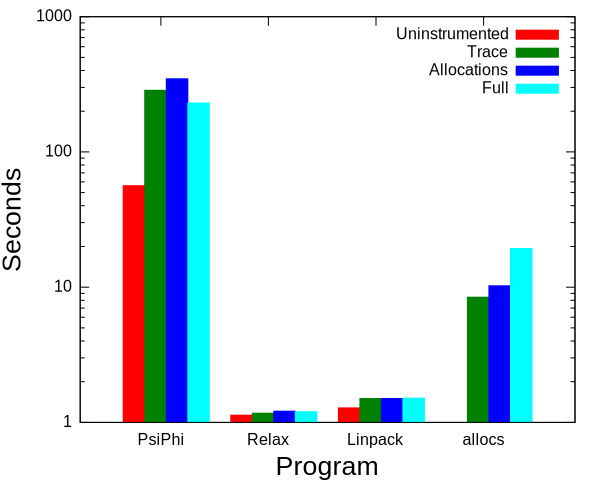
\includegraphics[width=\linewidth]{images/dbg/mtrace/performance}

  \caption{Performance of our evaluation programs under different
  instrumentation scenarios. Note logarithmic scale.  `Uninstrumented'
  is the runtime of the simulation without our interference. `Trace'
  interrupts for allocations; `Allocations' \emph{reports} allocations
  as well, which requires reading more data from the instrumented
  program.  `Full' does allocation tracking, access detection,
  analysis, and visualization of the data.}

  \label{fig:performance}
\end{figure}

Figure~\ref{fig:performance}'s `Relax' and `allocs' are artificial
programs constructed to illustrate overheads.  The
main component of `Relax' is Listing~\ref{lst:relaxation}. `allocs'
does nothing but allocate memory, the worst case for our
instrumentation.  We note that real-world programs experience
considerably lower overheads, with the popular Linpack seeing a modest
15\% slowdown.

\textit{Linpack} is the matrix-vector multiplication benchmark of
floating point performance that is used to rank supercomputers in the
popular `Top500' list. \textit{Relax} is a program that identifies
the steady state for the case of a plane connected to a constant heat
source.  The program's ratio between function calls and accessing the
data to be visualized is at parity, stressing the memory access and
analysis aspects of our supervisor. \textit{PsiPhi} is a real-world
computational fluid dynamics solver that focuses on Large Eddy
Simulation (LES) of flows that include combustion and other types of
chemical reactions~\cite{Proch:2014:PsiPhi}. \textit{allocs} is a test
program that simply allocs and frees memory without ever acessing it.

`Allocations' is a more expensive variant of the `Trace' benchmark.
In addition to allocation interception, this version reads relevant
information from the client process so that it may generate a report
of the [de]allocations made by the process.  The traces this algorithm
creates might be useful in producing and analyzing heap usage over
time, in the same manner as Valgrind's
`Massif'~\cite{Nethercote:2006:Massif}.  We note that this adds little
additional overhead to the instrumentation, demonstrating that reading
memory from the process is cheap.

%`Full' in
%Figure~\ref{fig:performance} details overheads for the full gamut of
%our analysis techniques.  Conflating the results, however, are filters
%that can be applied when more analysis is performed.  As one example of
%these
%filters, `Full' identifies the caller of \texttt{malloc} and ignores
%the allocation if the
%memory is an internal \textit{glibc} buffer.  With the extra
%information gained from this additional work, `Full' can in many
%cases realize that an allocation region is not interesting.  It then
%removes the item from the set of memory it tracks, thereby reducing the
%overhead induced.  If the overhead of tracking the memory exceeds that
%of the analysis, then this variant will actually be cheaper than the
%more na\"ive implementations.

In practical terms, the performance scales with 1) the number of
allocations the program performs, and 2) the number of allocations that
are tracked and provide source locations for analysis.  Reducing the
number of allocations requires changing the programs of interest, which
is counter to our goal of a transparent solution.  However, avoiding
the tracking infrastructure for memory that the user is not interested
in is a plausible practical mechanism by which the user can influence
the performance of the instrumented system.

%\section{Related work}
%
%Debugging high-performance computing applications is especially important as
%parallelism increases and debugging becomes correspondingly more difficult.
%\cite{Laguna:2011:Debugging} extend their earlier
%work~\cite{Bronevetsky:2010:AutomaDeD} with a scalable method to
%identify divergent parallel processes based on reduced control flow and
%call stack information. Gao et al.~\cite{Gao:2007:DMTracker} watch
%data movement patterns of a parallel application and use anomalies to
%statistically infer a set of undesirable program activites.
%\cite{Luecke:2003:MPICheck} instruments an MPI program to detect
%invalid or inconsistent usage of the library.  All of these debugging
%techniques are focused on identifying and eliminating the source of
%programming-level errors, such as data corruption, deadlock, or
%livelock.  In contrast, our \textit{ad hoc} visualization approach
%would be more appropriate to identify algorithmic errors, such as
%non-convergent error smoothing.
%
%\cite{Rosenblum:2011:Authors} use program control flow graphs and a
%custom-defined set of stylistic considerations to classify programs by
%their authors given only the input binary.
%\cite{Bernat:2012:BinEdit} define a number of `safe' control flow graph
%transformations and an algebra for describing and deriving new ones.
%Our code injection for page-aligned allocation is straightforward and
%undeserving of such a robust formalism.
%
%Our approach must identify and verify memory regions and related
%variables that meet a set of invariants. McCloskey et
%al.~\cite{McCloskey:2010:Infer} provided both a language and an
%implementation to specify complex invariants suitable for our analyses.
%\cite{Nguyen:2012:Invariants} use dynamic analysis to identify detailed
%invariants that include array accesses.  Our approach utilizes
%invariants that include reasoning at different levels, such as control
%flow, in addition to invariants like those discovered therein.
%\cite{Sharma:2013:DDEC} implement equivalence identification for
%instruction-level loops.  Our code injection and access detection might
%be seen as a lighter weight variant of their sandboxing technique.  The
%techniques in~\cite{Sharma:2013:DDEC} present a potential vector
%for inferring bounds from pointer-based loop guards, by deriving
%equivalent index-based guards and relying on our existing analysis
%infrastructure.

\section{Conclusions}

We have elucidated a method and demonstrated a prototype that
eliminates the surface area between simulation code and visualization
tool.  By recovering the loop structure of a target binary and
carefully instrumenting memory accesses, one can automatically insert
visualization at appropriate places in a running simulation.

%The major drawbacks at present are related to data types and data
%decomposition.  Presently we support only a single kind of simulation
%data: $N$-dimensional arrays.  While these have proven popular,
%they are far from universal.  Extending to other data types may be
%nontrivial.  A larger problem is data decomposition: we do not consider
%distributed-memory parallel simulations at present, and it seems likely
%that automatically reconstructing the full domain from its distributed
%pieces is undecidable.  User annotations may help in this endeavor.

\subsection{Future work}

The most glaring present omission is the lack of support for data
types beyond regular $N$-dimensional grids.  An obvious next target
is related data types such as adaptive mesh refinement data.
Curvilinear grids may prove simple as well, and meshes or point clouds
would certainly be of interest.  An area of uncertainty is in data
decomposition in distributed memory simulations.

We do not seek to replicate the full functionality of tools like
VisIt or ParaView.  We must therefore couple with one of these tools;
doing so would immediately increase the utility of our prototype
implementation.

We make a number of assumptions that are practically but not strictly
true.  Each requires more investigation, and aspects such as the
specification used in our search require more user control than we
presently have made available.

While some of these issues involve significant engineering efforts,
the work presented here demonstrates that there is no need to modify
simulation code to
inject \textit{in situ} visualization.  We hope this encourages others
to pursue 0-modification approaches to \textit{in situ} visualization.

%The astute reader may note that memory protection is possible only on
%page-aligned data.  We therefore require a modified \texttt{malloc}
%implementation that calls \texttt{posix\_memalign} (to allocate the
%page-aligned memory) followed by \texttt{mprotect} (to set up the
%desired memory protections).  Since we do not require the user to link
%against any runtime, adding a function in the traditional way is not
%viable.  Instead, we inject our modified \texttt{malloc} implementation
%directly into the executing process image after static initialization
%has completed.  We modify the instruction pointer when a
%\texttt{malloc} occurs to instead jump to our page protection
%allocation routine.

%\section{Related work}
%
%\textit{In situ} visualization has a rich history in the visualization
%community.  Recent frameworks include Damaris/Viz, the ParaView
%Coprocessing library, and VisIt's `libsim'~\cite{Dorier:2013:Damaris,
%Fabian:2011:Catalyst, Whitlock:2011:Libsim}. Dorier et
%al.~\cite{Dorier:2013:Damaris} open
%by noting the important factors for an \textit{in situ} visualization
%tool. Among these factors are \textbf{low impact on code} and
%\textbf{low impact on runtime}.  As our solution requires zero code
%modifications, it has the lowest impact on the simulation code of any
%\textit{in situ} visualization tool.  Performance is viable in
%favorable conditions, and we hope to lower the overhead in the future.
%
%Debugging high-performance computing applications is especially important as
%parallelism increases and debugging becomes correspondingly more difficult.
%\cite{Laguna:2011:Debugging} extend their earlier
%work~\cite{Bronevetsky:2010:AutomaDeD} with a scalable method to
%identify divergent parallel processes based on reduced control flow and
%call stack information. Gao et al.~\cite{Gao:2007:DMTracker} watch
%data movement patterns of a parallel application and use anomalies to
%statistically infer a set of undesirable program activites.
%\cite{Luecke:2003:MPICheck} instruments an MPI program to detect
%invalid or inconsistent usage of the library.  All of these debugging
%techniques are focused on identifying and eliminating the source of
%programming-level errors, such as data corruption, deadlock, or
%livelock.  In contrast, our \textit{ad hoc} visualization approach
%would be more appropriate to identify algorithmic errors, such as
%non-convergent error smoothing.
%
%\cite{Rosenblum:2011:Authors} use program control flow graphs and a
%custom-defined set of stylistic considerations to classify programs by
%their authors given only the input binary.
%\cite{Bernat:2012:BinEdit} define a number of `safe' control flow graph
%transformations and an algebra for describing and deriving new ones.
%Our code injection for page-aligned allocation is straightforward and
%undeserving of such a robust formalism.
%
%Our approach must identify and verify memory regions and related
%variables that meet a set of invariants. McCloskey et
%al.~\cite{McCloskey:2010:Infer} provided both a language and an
%implementation to specify complex invariants suitable for our analyses.
%\cite{Nguyen:2012:Invariants} use dynamic analysis to identify detailed
%invariants that include array accesses.  Our approach utilizes
%invariants that include reasoning at different levels, such as control
%flow, in addition to invariants like those discovered therein.
%\cite{Sharma:2013:DDEC} implement equivalence identification for
%instruction-level loops.  Our code injection and access detection might
%be seen as a lighter weight variant of their sandboxing technique.  The
%techniques in~\cite{Sharma:2013:DDEC} present a potential vector
%for inferring bounds from pointer-based loop guards, by deriving
%equivalent index-based guards and relying on our existing analysis
%infrastructure.


\chapter{Conclusions and future work}
\label{chp:conclusions}
lorem ipsum dolor sit amet
%* in situ vis
%	* approaching: do sim for every new vis/analysis question


\bibliographystyle{unsrt}
\bibliography{alt,analysis,compositing,insitu,iorefs,understanding,us,vr,vis}

\end{document}
